\documentclass[letterpaper, 10 pt, conference]{ieeeconf}  % Comment this line out if you need a4paper

\IEEEoverridecommandlockouts                             
\overrideIEEEmargins

\usepackage[utf8]{inputenc}
\usepackage[T1]{fontenc}
\usepackage{graphicx}
\usepackage{float}
\usepackage{xcolor}

\usepackage{amsmath}
\usepackage{amsfonts}
\usepackage{amssymb}
\usepackage{mathtools}

\newcommand{\ph}[1]{{\textbf{#1}:}} % paragraph header
\newcommand{\todo}[1]{{\color{red} #1 }} % Tasks to do
\newcommand{\note}[1]{{\color{cyan} NOTE: #1 }}

\newcommand{\argmax}{\mathop{\mathrm{argmax}}}
\newcommand{\argmin}{\mathop{\mathrm{argmin}}}


\title{\LARGE \bf
Perception-aware and Risk-cognizant Planning Under Uncertainty for Autonomy in Extreme Environments
}


\begin{document}
\maketitle
\thispagestyle{empty}
\pagestyle{empty}


\begin{abstract}
In this work, we propose a framework for planning under uncertainty that bridges the gap between high-fidelity continuous traversability analysis and discrete behavior planning.
\end{abstract}


%%%%%%%%%%%%%%%%%%%%%%%%%%%%%%%%%%%%%%%%%%%%%%%%%%%%%%%%%%%%%%%%%%%%%%%%%%%%%%%%
\section{Instructions}
\ph{Paragraph header} Please start every single paragraph with a paragraph header, summarizing the intention of that paragraph. This is mainly for iterations during the paper preparation. We will remove most of them for the final report.

%%%%%%%%%%%%%%%%%%%%%%%%%%%%%%%%%%%%%%%%%%%%%%%%%%%%%%%%%%%%%%%%%%%%%%%%%%%%%%%%
\section{Introduction}
\ph{Real world example} Consider a robot tasked to explore and search a GPS-denied environment, under given time constraints. Creating a map of the environment, accurately predicting risks, and planning motions that can meet the coverage and time requirements are essential elements of autonomy architecture to realize such a mission.
... discuss uncertainty...

\todo{[Amanda] Add a nice figure at the top right}

\ph{Generic formulation}
The above-mentioned mission in its most general form can be cast as a ...

\ph{Gap in the state-of-the-art}
The current methods .... However, when it comes to ... 

\ph{Contributions}
In this work, we ...

\ph{Outline}
In the next section, we will ...


%%%%%%%%%%%%%%%%%%%%%%%%%%%%%%%%%%%%%%%%%%%%%%%%%%%%%%%%%%%%%%%%%%%%%%%%%%%%%%%%
\section{Related Work}

%%%%%%%%%%%%%%%%%%%%%%%%%%%%%%%%%%%%%%%%%%%%%%%%%%%%%%%%%%%%%%%%%%%%%%%%%%%%%%%%
\section{Problem Formulation}

In this section, we formulate our autonomous exploration problem for DARPA Subterranean (SubT) Challenge.
At a high level, the objective is to \textit{detect} and \textit{localize} the artifact objects in an unknown environment as many as possible for the given time.
Note that this is a highly complex problem that requires simultaneous perception, localization, mapping, and planning for the optimal solution.

\subsection{Belief State Representation}

In this section we briefly introduce generic POMDP formulation.
For a detailed information, see e.g.,~\cite{Bertsekas05,TBF05,RN10}.

Let $\mathbb{S}$, $\mathbb{A}$, and $\mathbb{Z}$ denote the state, action, and observation spaces, respectively.
We denote the motion model $T(s, a, s') = P(s'\,|\,s, a)$, which defines the probability of being at state $s'$ after taking an action $a$ in state $s$.
The observation model $Z(s, a, z) = P(z\,|\,s, a)$ is the probability of receiving observation $z$ after taking action $a$ in state $s$. 

A belief $b(s)$ is a posterior distribution over all possible states given the past actions and observations, i.e., $b_{t}(s) = P(s \,|\, a_{0:t-1}, z_{1:t})$ where the subscript $t$ denotes the time step.
Note that a POMDP problem can be formulated as a \textit{Belief MDP} by taking $b(s)$ as an MDP state, also referred to as a \textit{belief state} $b \in \mathbb{B}$, where $\mathbb{B}$ is referred to as \textit{belief space}.

Given $a_{t-1}$, $z_t$, and $b_{t-1}(s)$,
the updated belief $b_t(s)$ can be computed by Bayesian filtering, which can be divided into two sub-steps as follows.
\begin{align}
  b_{t-1}(s; a_{t-1}) &= \sum_{s' \in \mathbb{S}} T(s, a_{t-1}, s') b_{t-1}(s),
  \label{eq:prediction}
  \\
  b_t(s; a_{t-1}, z_t) &= \eta Z(s, a_{t-1}, z_t) b_{t-1}(s; a_{t-1}),
  \label{eq:correction}
\end{align}
where $\eta$ is a normalizing constant.
% For notational convenience, let us denote $b_{t-1}(s; a) = b_{t-1}^a$ and $b_t(s; a, z) = b_t = b_{t-1}^{a z}$ hereafter.

A policy $\pi : \mathbb{B} \rightarrow \mathbb{A}$ maps each belief state $b$ to a desirable action $a$.

\subsection{Global Optimization Problem}

As briefly mentioned above, the overall objective of our problem is to detect and localize the artifact objects in an unknown environment.  We first define a belief state of the problem for the POMDP formulation:
\begin{align}
  b \in \mathbb{B} = p(M, x),
\end{align}
where $M$ represents a map, and $x$ stands for the current robot pose.
Note that a Rao-Blackwellized particle filter can be used to represent $b$ by a set of sampled states drawn from $p(M, x)$ \cite{stachniss2005information}.

Our goal is to find optimal actions to take which maximize the information gained from the environment.  Informally, let $I(b, \pi(b))$ denote the information gain about the occupancy grid map states and robot localization after taking an action at $b$ under $\pi$.  We will formally define $I$ in subsequent sections; for now we are concerned with formulating this objective as an optimization problem to maximize the information gain from the environment:
\begin{align}
  J(b;\pi) &= \mathbb{E} \left[ \sum_{t=0}^\infty \gamma^t I(b_t; \pi_t(b_t)) \right], \label{eq:artifactopt_cost}\\
  \pi^*(b) & = \argmax_{\Pi} J(b;\pi), \label{eq:artifactopt}\\
  J^*(b) &= \max_{\Pi} J(b;\pi) , \label{eq:artifactopt_value}\\
\end{align}

% \note{Here, we do not explicitly include the localization accuracy in the objective function, unlike some of SLAM formulations. If anyone has a good idea how to describe this, please feel free to contribute.}

where $J(b;\pi)$ is the value function and $J^*(b)$ is the optimal value function.  Traditionally, this problem can be solved at each timestep using a dynamic programming approach, which decomposes the maximization over an infinite number of timesteps to a maximization over one timestep at a time.  We can rewrite Eq.~(\ref{eq:artifactopt_value}) in a recursive form, which is called the optimal Bellman equation.
\begin{align}
J^*(b) = \max_{\Pi} \left[I(b, \pi(b)) % \nonumber \\
   + \gamma \sum_{b' \in \mathbb{B}} \tau(b, \pi(b), b') J^*(b')\right],
  \label{eq:bellman}
\end{align}
where $\tau(b, \pi(b), b') = \sum_{z \in \mathbb{Z}} P(b'|b,\pi(b),z) P(z|b,\pi(b))$ is the transition probability from $b$ to $b'$ under $\pi$,
which can be derived from Eq.~(\ref{eq:prediction}) and~(\ref{eq:correction}).
For further details, see~\cite{Ross08}.

% It is often convenient to define the so-called Q-value function for an intermediate belief-action pair, $(b, a)$ or simply $b^a$, as follows.
% \begin{align}
%   Q(b, a; \pi) =\; & I(b, a) + \gamma \sum_{b' \in \mathbb{B}} \tau(b, a, b') J(b'; \pi).
%   \label{eq:qfunction}
% \end{align}
% Then Eq.~(\ref{eq:bellman}) can be written as:
% \begin{align}
% J(b; \pi) =\; & \min_{a \in \mathbb{A}} Q(b, a; \pi)
% \label{eq:minq}
% \end{align}

However, because in our setting we aim to tackle problems which have large time horizons (>1 hour), large spatial extents (>10km$^2$), and high dimensional belief states, determining $J^*$ over the full belief $b=p(M,x)$ becomes intractable.  Therefore we introduce several key spatial and temporal decompositions which restrict the class of pol

\subsection{Problem Decomposition}

We introduce a three-stage decomposition of the problem to arrive at a tractable approximation of the globally optimal solution.  We decompose Eq. (\ref{eq:occupancyopt}) as follows:

\begin{align}
  \pi_{0:T}^*(b)
  & = \argmax_{\Pi_{0:T}} \mathbb{E} \left[ \sum_{t=0}^T I^M(b_t; \pi_t(b_t)) \right]
  \label{eq:globalopt}
  \\
  & \approx \sum_{t=0}^T \argmax_{\Pi_{t}} \mathbb{E} \left[ \frac{I^M(b_t; \pi_t(b_t))}{c_t^M(b_t; \pi_t(b_t))} \Delta t \right]
  \label{eq:recedinghorizon}
  \\
  & \approx \sum_{t=0}^T \pi_b^{G*}(b) \Delta t.
  \label{eq:hierarchical}
\end{align}
Note that we approximated Eq.~(\ref{eq:globalopt}) to Eq.~(\ref{eq:recedinghorizon}) based on receding horizon planning scheme, and Eq.~(\ref{eq:recedinghorizon}) to Eq.~(\ref{eq:hierarchical}) based on hierarchical optimization scheme. 
\todo{[Amanda] add architecture figure}



We can also define an artifact grid map $\tilde{M}$ and a corresponding belief state $\tilde{b}$ as follows.
\begin{align}
  \tilde{M} &= (\tilde{\mathbf{m}}^1, \tilde{\mathbf{m}}^2, \dots, \tilde{\mathbf{m}}^{N_M}), \\
  \tilde{b} &= p(\tilde{M}, x),
\end{align}
where $\tilde{\mathbf{m}}^i$ is a Bernoulli random variable for the binary artifact existence state of the $i$-th cell,
i.e., $\tilde{\mathbf{m}}^i \in \{existent, nonexistent\}$.
\note{We can extend this notation to consider more details related to artifact detection/perception.}


Notice that $I^A(\tilde{b}, \pi(\tilde{b}))$ in Eq.~(\ref{eq:artifactopt}) implicitly depends on the performance of the perception module, i.e., the artifact object detection module.
In this work, we assume that the artifact object detection works perfectly, and decouple perception from our optimization framework.
In other words, we assume all artifact objects will be detected if the occupancy grid map has been fully covered.
\note{We can further incorporate artifact detection in our framework to some extent.}

Then, we can rewrite the optimization problem as follows.
\begin{align}
  \pi_{0:T}^*(b) & = \argmax_{\Pi_{0:T}} \mathbb{E} \left[ \sum_{t=0}^T I^M(b_t; \pi_t(b_t)) \right],
  \label{eq:occupancyopt}
\end{align}
where $I^M(b, \pi(b))$ is the information gain about the occupancy grid map states and robot localization after taking an action at $b$ under $\pi$.

%%%%%%%%%%%%%%%%%%%%%%%%%%%%%%%%%%%%%%%%%%%%%%%%%%%%%%%%%%%%%%%%%%%%%%%%%%%%%%%%
\section{Proposed Framework}

In this section, we propose a \emph{receding-horizon hierarchical optimization} framework to tackle our simultaneous localization, mapping, and planning problem.
We first introduce Information Roadmap (IRM) which is a sparse graph that encodes the connectivity of the free space in the environment and other abstract information such as node-to-node traversability.
Then we describe the receding-horizon hierarchical optimization framework for autonomous exploration in large unknown environments.


\subsection{Information Roadmap (IRM)}

\todo{TODO}
\todo{[Amanda] Add a nice IRM figure}


\subsection{Receding-horizon Hierarchical Optimization}

We employ two strategies to solve our optimization problem; receding-horizon planning and hierarchical optimization.
%
Due to the curse of history in POMDPs, the problem complexity increases exponentially with the planning horizon \cite{Pineau03}.
Receding-horizon planning is a common scheme to tackle such a challenge by interleaving execution and replanning for a finite horizon.
%
Hierarchical optimization is also a useful methodology to solve large-scale problems in accordance with the divide-and-conquer paradigm.
\todo{TODO: add references for each.}

Our proposed framework is composed of receding-horizon planners in three hierarchical levels--graph, map, and traversability levels.
Graph-level planning is conducted on the IRM, using the embedded information in its nodes and edges.
Map-level planning uses a local occupancy grid map (20m$\times$20m) that is centered at the current robot pose.
Traversability-level planning uses a smaller local occupancy grid map (5m$\times$5m) and the corresponding point cloud sensor data for the robot-specific traversability analysis.
In order to ensure the robots continue autonomous exploration over time, we additionally impose a constraint regarding the risk level on each optimization problem.


\subsubsection{Graph-level Receding-horizon Planning}

\begin{align}
  \pi_t^{G*}(b) &= \argmax_{\Pi_t^G} \mathbb{E} \left[ \frac{I^G(b; \pi_t^G(b))}{c_t^G(b; \pi_t^G(b))} \right]
  \nonumber \\
  s.t.~&~\rho_t^G(b; \pi_t^G(b))< \psi^G(t).
  \label{eq:graphopt}
\end{align}
where $I^G(b; \pi_t^G(b))$ is the information gain in the graph level,
$c_t^G(b; \pi_t^G(b))$ is a cost function that returns a time to execute an action under $\pi_t^G$.
$\rho_t^G(b; \pi_t^G(b))$ is a risk measure for taking an action at $b$ under $\pi_t^G$, and
$\psi^G(t)$ is a time-varying threshold for allowable risk at time $t$.
(For example, $\psi^G(t)$ gets higher as $t$ gets closer to $T$, the total allowed time for exploration, in order to allow riskier actions.)

We define the graph-level policy as follows.
\begin{align}
  \pi_t^G(b) = 
  \begin{dcases*}
    \pi_t^{M*}(b; F^d) & if $b \in \mathbb{N}(F^d)$ \\
    a_t^G(b; F^d) & otherwise 
  \end{dcases*},
\end{align}
where $F^d$ is the desired frontier cluster (\todo{TODO: need more explanation}\!\!) based on $\pi_t^G$, and
$\mathbb{N}(F^d)$ stands for the neighborhood belief states of $F^d$.
$\pi_t^{M*}(b; F^d)$ is an optimal policy in the map level for $b$ given $F^d$, and
$a_t^G(b; F^d)$ is an abstract graph-level action to reach $F^d$ following the shortest path IRM edges.
\note{We may add another low-level optimization that solves for the concrete robot trajectory $x_{0:k}$ for the given $a_t^G$, which is effectively the mobility service in our implementation.}


\subsubsection{Map-level Receding-horizon Planning}

\begin{align}
  \pi_t^{M*}(b; F^d) &= \argmax_{\Pi_t^M} \mathbb{E} \left[ \frac{I^M(b; \pi_t^M(b; F^d))}{c_t^M(b; \pi_t^M(b; F^d))} \right]
  \nonumber \\
  s.t.~&~\rho_t^M(b; \pi_t^M(b; F^d))< \psi^M(t).
  \label{eq:mapopt}
\end{align}
where the notations are the same with Eq.~(\ref{eq:graphopt}) except that those with the superscript $M$ are for the map level.

Similarly, we define the map-level policy as follows.
\begin{align}
  \pi_t^M(b; F^d) = \pi_t^{T*}(b; F^d, x^d),
\end{align}
where $x^d$ is the desired robot pose based on $\pi_b^M$.


\subsubsection{Traversability-level Receding-horizon Planning}

\begin{align}
  \pi_t^{T*}(b; F^d, x^d)
  &= \argmin_{\Pi_t^T} \mathbb{E} \left[ c^T(b; \pi_t^T(b; F^d, x^d)) \right]
  \nonumber \\
  s.t.~&~\rho_t^T(b; \pi_t^T(b; F^d, x^d))< \psi^T(t).
  \label{eq:travopt}
\end{align}
where the notations are the same with Eq.~(\ref{eq:graphopt}) except that those with the superscript $T$ are for the traversability level.

The traversability-level policy returns a desired robot trajectory $x_{t, 0:K}$, where the subscript $k$ denotes the time sub-step, dividing a single time step between $t$ and $t+1$ by $K$ sub-steps.

The cost function in this level can be defined as follows.
\begin{align}
  c^T(b; \pi_t^T(b; F^d, x^d)) = c_l \sum_{k=0}^{K-1} d(x_k, x_{k+1}) + c_\rho \sum_{k=0}^K \rho_t^T(x_k),
\end{align}
where $d(x_k, x_{k+1})$ is a distance measure between two poses, $x_k$ and $x_{k+1}$.
$c_l$ and $c_\rho$ are the weights for the path length and the risk measure, respectively.


%%%%%%%%%%%%%%%%%%%%%%%%%%%%%%%%%%%%%%%%%%%%%%%%%%%%%%%%%%%%%%%%%%%%%%%%%%%%%%%%
\section{Future Work}


- [local] lower-level planning for local search

- [local] multi-step look-ahead planning

- [local] leaf node value estimation (prior/heuristic/learn-ing)

- [global] multi-step look-ahead planning




\clearpage
%%%%%%%%%%%%%%%%%%%%%%%%%%%%%%%%%%%%%%%%%%%%%%%%%%%%%%%%%%%%%%%%%%%%%%%%%%%%%%%%
\section{Problem Formulation}
Let $s$, $\pi_f$, and $M$ denote the robot's state, a move-to-frontier action, and map, respectively. We formulate the coverage objective function as the ratio of newly sensed map information ($B$) to the temporal cost of sensing this information ($c_t$), both of which are functions of the transition function $T(s,\pi_f,M)$.

\begin{align}
    J^{cov}(s,\pi_f,M) &= \frac{B[T(s,\pi_f,M)]}{c_t[T(s,\pi_f,M)]} \\ \nonumber \\ 
    T &\colon s \times \pi_f \times M\to \tau \nonumber \\
    B &\colon \tau\to \Delta n_{bc} \nonumber \\
    c_t &\colon s \times \pi_f \times M\to \Delta t \nonumber 
\end{align}

\noindent where, for a given the move-to-frontier action $\pi_f$, $\tau$ is the robot trajectory, $\Delta t$ is duration of traversal, and $\Delta n_{bc}$ is the number of new breadcrumbs added to the IRM. We select an action $\pi_f$ which maximizes our coverage objective function:
\begin{align}
    % f^* &= \arg\max_{f\in F}_{~~\tau \in \Gamma} J^{cov}(s,f,M) \\
    \pi_f^* &= \arg\max_{\substack{\pi_f\in \Pi_f \\ \tau \in T}} J^{cov}(s,f,M) \\
    s.t.~~&~\textrm{risk}(s,\pi_f,M)< \psi(t)
\end{align}

\noindent The risk (or probability of traversal) associated with the optimal action is required to be smaller than a time adaptive threshold. As the duration of the mission progresses, the risk threshold $\psi(t)$ increases to allow for riskier actions.

% Let $x_k$, $u_k$, and $z_k$ denote the robot state, action, and observation at the $k$-th time step.
% \begin{align}
%     \pi^* &= \arg\min_{\pi\in \Pi} J(?, ?, \pi) \\
%     s.t.~~&~constraint 1 \\
%     ~ &~constraint 2
% \end{align}

\subsection{Defining risk}
It is easier to define risk as the probability of success, rather than the probability of failure, since for the mission to succeed, we require the intersection of multiple successful events.  Let $r(s,\pi_f,M,t)$ be the probability of success associated at each (timestep?  transition?), which we define as the probability that the robot does not fail or crash for that interval.  We define the total \emph{mission risk} $R$ as the probability that the robot does not fail over the entire mission.  For a given mission duration $D$, the mission risk is given by:
\begin{equation}
    R= \prod_{t=0}^D risk(s,\pi_f,M,t)
\end{equation}
In general, risk may be a function of the state $s$, actions $\pi_f$, and map $M$.  We can make the simplifying assumption that is is a function each grid cell within the map $m_i$.  (is $m_i$ the occupancy value or the grid itself?  or is $i$ indication the grid?)  Let $m_i(t)$ be the grid cell that the robot occupies at time $t$.  Then we have $risk(m_i(t)) = \prod_{k} r_k(m_i(t))$ where we have $k$ risk factors.  Each risk factor may be due to a different source of potential failure, e.g. rough terrain, proximity to obstacles, slope, slippery/muddy terrain, etc.  For computational tractability we can compute the log mission risk: 
\begin{equation}
    \log R=\bigg[\sum_{t=0}^D\sum_{k} \log(r_k(m_i(t)))\bigg] > \Phi
\end{equation}
which we want to constrain to be above some total acceptable mission risk threshold $\Phi$.
\section{Problem Solution}

\subsection{Local Selection}

\begin{itemize}
  \item Objective 1: Connect local to global coverage
  \begin{itemize}
  \item In-depth path planning to selected frontier
  \item Expectation Model or leaf-node heuristic function
  \end{itemize}
  \item Objective 2: More robust traversability (no oscillations!)
  \begin{itemize}
  \item Way-point assignments 
  \end{itemize}
\end{itemize}


%%%%%%%%%%%%%%%%%%%%%%%%%%%%%%%%%%%%%%%%%%%%%%%%%%%%%%%%%%%%%%%%%%%%%%%%%%%%%%%%
\section{Environment representation}
\subsection{Occupany Grid Mapping}
Given a set of observations taken at known robot poses, the posterior over maps is given by:
\begin{align}
    p(m | z_{1:t},x_{1:t})
\end{align}
\noindent where $m$ is the map, $z_{1:t}$ is the set of all measurements up to time $t$, and $x_{1:t}$ is path of robot. 
Occupancy grid map is composed of grid cells:
\begin{align}
    m = \{\textbf{m}_i\}
\end{align}
\noindent where $\textbf{m}_i$ is associated with a binary occupancy value indicating whether cell is occupied or free. Calculating the posterior for every single map is intractable, therefore, problem can be formulated as the posterior over a single grid cell: 
\begin{align}
    p(\textbf{m}_i | z_{1:t},x_{1:t})
\end{align}
Here, we are estimating a fixed, binary state that does not change over time. When the state is static, posterior is only function of measurements:
\begin{align}
    p(\textbf{m}_i | z_{1:t},x_{1:t}) = p(\textbf{m}_i | z_{1:t})
    \label{static}
\end{align}
This problem can be addressed by the Binary Bayes filter. The \emph{odds} of a state $\textbf{m}_i$ is defined as the ratio of the probability that the cell is free to that of the cell being occupied:
\begin{align}
    \frac{p(\textbf{m}_i | z_{1:t},x_{1:t})}{1-p(\textbf{m}_i | z_{1:t},x_{1:t})}
    \label{odd}
\end{align}
The \emph{log odds} is the logarithm of this ratio:

\begin{align}
    l_{t,i} = \log\frac{p(\textbf{m}_i | z_{1:t},x_{1:t})}{1-p(\textbf{m}_i | z_{1:t},x_{1:t})}
    \label{log_odd}
\end{align}
An inverse measurement model, $p(\textbf{m}_i | z_{1:t},x_{1:t})$, which specifies the distribution over the binary state variable $\textbf{m}_i$ as a function of the measurement $z_{1:t}$, is used since the measurements are much more complex than the binary state. 
\noindent By rearranging Eq.~(\ref{log_odd}), the posterior over the grid cell is exposed:
\begin{align}
    p(\textbf{m}_i | z_{1:t},x_{1:t}) = 1-\frac{1}{1+\exp(l(\textbf{m}_i))}
\end{align}
\noindent Eq.~(\ref{log_odd}) can be expanded in accordance with Bayes filter:
\begin{align}
    l_{t,i} &= \log\frac{p(\textbf{m}_i | z_{1:t-1}, x_{1:t-1})}{1-p(\textbf{m}_i | z_{1:t-1}, x_{1:t-1})} + \log\frac{p(\textbf{m}_i | z_{t},x_{t})}{1-p(\textbf{m}_i | z_{t},x_{t})} \nonumber \\
    &\quad - \log\frac{p(\textbf{m}_i)}{1-p(\textbf{m}_i)} \nonumber \\
    &= l_{t-1,i} + \log\frac{p(\textbf{m}_i | z_{t},x_{t})}{1-p(\textbf{m}_i | z_{t},x_{t})} - l_{0,i}
\end{align}
\noindent where $l_{t-1,i}$ is the previous log-odds value, $l_{0,i}$ is the log-odds representation of the occupancy prior $p(\textbf{m}_i)$, and $p(\textbf{m}_i | z_{t},x_{t})$ is the inverse sensor model.

However, this formulation does not reflect dependencies among neighboring cells. 

\subsection{Information Gain}
Entropy is a measure for the uncertainty of a posterior. The entropy $H_p(x)$ of a probability distribution $p$ is the expected information $E[-\log p]$. The entropy of the occupancy grid map posterior is
\begin{align}
    H_p(\textbf{m}_i) = -p(\textbf{m}_i) \log p(\textbf{m}_i) - (1-p(\textbf{m}_i)) \log(1-p(\textbf{m}_i))
\end{align}
\noindent and the expected entropy after measuring is $E[H_{p}(\textbf{m}_i)]$. Then the expected information gain when sensing a grid cell $\textbf{m}_i$ is: 
\begin{align}
    I_i = H_p(\textbf{m}_i) - E[H_{p}(\textbf{m}_i)]
\end{align}



%%%%%%%%%%%%%%%%%%%%%%%%%%%%%%%%%%%%%%%%%%%%%%%%%%%%%%%%%%%%%%%%%%%%%%%%%%%%%%%%
\section{Risk quantification}
In this section, we discuss how we associate risk and cost values to a given trajectory in the environment.

%%%%%%%%%%%%%%%%%%%%%%%%%%%%%%%%%%%%%%%%%%%%%%%%%%%%%%%%%%%%%%%%%%%%%%%%%%%%%%%%
\section{Frontier-based Coverage Planning}

\subsection{IRM}



\subsection{Frontier Detection}

\subsubsection{Frontier map}
\todo{David} How we represent 3D lidar data in 2D frontier map
\begin{itemize}
    \item We want to capture traversability information here
    \item We can include a full discussion about traversability analysis, computing risk metrics for traversal, and capturing known vs. unknown regions
    \item We can fold in the current writeup on traversability here, then add additional risk/traversability metrics
\end{itemize}
\subsubsection{Frontier detection}
\todo{Sung} Frontier detection algorithm


\subsection{Frontier Maintenance}
\todo{Sung} Frontier node maintenance details

%%%%%%%%%%%%%%%%%%%%%%%%%%%%%%%%%%%%%%%%%%%%%%%%%%%%%%%%%%%%%%%%%%%%%%%%%%%%%%%%
\section{Experiments}


%%%%%%%%%%%%%%%%%%%%%%%%%%%%%%%%%%%%%%%%%%%%%%%%%%%%%%%%%%%%%%%%%%%%%%%%%%%%%%%%
\section{Conclusion}




% %%%%%%%%%%%%%%%%%%%%%%%%%%%%%%%%%%%%%%%%%%%%%%%%%%%%%%%%%%%%%%%%%%%%%%%%%%%%%%%%
% \section{Instructions}
% \ph{Paragraph header} Please start every single paragraph with a paragraph header, summarizing the intention of that paragraph. This is mainly for iterations during the paper preparation. We will remove most of them for the final report.

% %%%%%%%%%%%%%%%%%%%%%%%%%%%%%%%%%%%%%%%%%%%%%%%%%%%%%%%%%%%%%%%%%%%%%%%%%%%%%%%%
% \section{Introduction}
% \ph{Real world example} Consider a robot tasked to map a GPS-denied area in moving under time constraints. 

% %%%%%%%%%%%%%%%%%%%%%%%%%%%%%%%%%%%%%%%%%%%%%%%%%%%%%%%%%%%%%%%%%%%%%%%%%%%%%%%%
% \section{Problem Formulation}
% Let $x_k$, $u_k$, and $z_k$ denote the robot state, action, and observation at the $k$-th time step.


% %%%%%%%%%%%%%%%%%%%%%%%%%%%%%%%%%%%%%%%%%%%%%%%%%%%%%%%%%%%%%%%%%%%%%%%%%%%%%%%%
% \section{Map Representation}


% %%%%%%%%%%%%%%%%%%%%%%%%%%%%%%%%%%%%%%%%%%%%%%%%%%%%%%%%%%%%%%%%%%%%%%%%%%%%%%%%
% \section{Something of Map Posterior}

% %%%%%%%%%%%%%%%%%%%%%%%%%%%%%%%%%%%%%%%%%%%%%%%%%%%%%%%%%%%%%%%%%%%%%%%%%%%%%%%%
% \section{Planning}

% %%%%%%%%%%%%%%%%%%%%%%%%%%%%%%%%%%%%%%%%%%%%%%%%%%%%%%%%%%%%%%%%%%%%%%%%%%%%%%%%
% \section{Experiments}


% %%%%%%%%%%%%%%%%%%%%%%%%%%%%%%%%%%%%%%%%%%%%%%%%%%%%%%%%%%%%%%%%%%%%%%%%%%%%%%%%
% \section{Conclusion}



\section*{APPENDIX}


%%%%%%%%%%%%%%%%%%%%%%%%%%%%%%%%%%%%%%%%%%%%%%%%%%%%%%%%%%%%%%%%%%%%%%%%%%%%%%%%
\section{Background}

\subsection{Partially Observable Markov Decision Process (POMDP)}

%% (excerpted from Sung's thesis)

In this section we briefly introduce generic POMDP formulation.
For a detailed information, see e.g.,~\cite{Bertsekas05,TBF05,RN10}.

Let $\mathbb{S}$, $\mathbb{A}$, and $\mathbb{Z}$ denote the state, action, and observation spaces, respectively.
We denote the motion model $T(s, a, s') = P(s'\,|\,s, a)$, which defines the probability of being at state $s'$ after taking an action $a$ in state $s$.
The observation model $Z(s, a, z) = P(z\,|\,s, a)$ is the probability of receiving observation $z$ after taking action $a$ in state $s$. 

A belief $b(s)$ is a posterior distribution over all possible states given the past actions and observations, i.e., $b_{t}(s) = P(s \,|\, a_{0:t-1}, z_{1:t})$ where the subscript $t$ denotes the time step.
Note that a POMDP problem can be formulated as a \textit{Belief MDP} by taking $b(s)$ as an MDP state, also referred to as a \textit{belief state} $b \in \mathbb{B}$, where $\mathbb{B}$ is referred to as \textit{belief space}.

Given $a_{t-1}$, $z_t$, and $b_{t-1}(s)$,
the updated belief $b_t(s)$ can be computed by Bayesian filtering, which can be divided into two sub-steps as follows.
\begin{align}
  b_{t-1}(s; a_{t-1}) &= \sum_{s' \in \mathbb{S}} T(s, a_{t-1}, s') b_{t-1}(s),
  \label{eq:prediction}
  \\
  b_t(s; a_{t-1}, z_t) &= \eta Z(s, a_{t-1}, z_t) b_{t-1}(s; a_{t-1}),
  \label{eq:correction}
\end{align}
where $\eta$ is a normalizing constant.
% For notational convenience, let us denote $b_{t-1}(s; a) = b_{t-1}^a$ and $b_t(s; a, z) = b_t = b_{t-1}^{a z}$ hereafter.

A policy $\pi : \mathbb{B} \rightarrow \mathbb{A}$ maps each belief state $b$ to a desirable action $a$.
The expected cost of an action for the true state can be represented as a cost function in a belief space, $c(b, a) \in \mathbb{R}^+$.
Given a policy $\pi$ and a belief $b \in \mathbb{B}$, we can compute the value function,
\begin{align}
  J(b; \pi) = \mathbb{E} \left[ \sum_{t=0}^\infty \gamma^t c(b_t, \pi(b_t)) \right]\!,
  \label{eq:trueV}
\end{align}
where $b_0$ is the initial belief state and 	$\gamma \in (0, 1]$ is a discount factor that reduces the effect of later costs.


We can rewrite Eq.~(\ref{eq:trueV}) in a recursive form, which is called the Bellman equation.
\begin{align}
J(b; \pi) = c(b^i, \pi(b)) % \nonumber \\
   + \gamma \sum_{b' \in \mathbb{B}} \tau(b, \pi(b), b') J(b'; \pi),
  \label{eq:bellman}
\end{align}
where $\tau(b, \pi(b), b') = \sum_{z \in \mathbb{Z}} P(b'|b,\pi(b),z) P(z|b,\pi(b))$ is the transition probability from $b$ to $b'$ under $\pi$,
which can be derived from Eq.~(\ref{eq:prediction}) and~(\ref{eq:correction}).
For further details, see~\cite{Ross08}.

It is often convenient to define the so-called Q-value function for an intermediate belief-action pair, $(b, a)$ or simply $b^a$, as follows.
\begin{align}
  Q(b^a; \pi) =\; & c(b, a) + \gamma \sum_{b' \in \mathbb{B}} \tau(b, a, b') J(b'; \pi).
  \label{eq:qfunction}
\end{align}
Then Eq.~(\ref{eq:bellman}) can be written as follows.
\begin{align}
J(b; \pi) =\; & \min_{a \in \mathbb{A}} Q(b, a; \pi)
\label{eq:minq}
\end{align}

We now restate our POMDP problem as an optimization problem.
\begin{align}
  \pi^*(b) & = \argmin_{\Pi_{0:\infty}} \mathbb{E} \left[ \sum_{t=0}^\infty \gamma^t c(b_t, \pi_t(b_t)) \right]
  \nonumber \\ 
  &  = \argmin_{\Pi_{0:\infty}} J(b_t; \pi_t).
  \label{eq:pomdpopt}
\end{align}


\subsection{Occupancy Grid Mapping}

An occupancy grid map is a discretized random field in multi-dimensional space, where each independent cell stores a probabilistic estimate of its occupancy state \cite{moravec1985high,elfes1990stochastic}.
%
Formally, an occupancy grid map is composed of grid cells:
\begin{align}
  M = (\mathbf{m}^1, \mathbf{m}^2, \dots, \mathbf{m}^{N_M}),
\end{align}
where $\mathbf{m}^i$ is a Bernoulli random variable for the binary occupancy state of the $i$-th cell,
i.e., $\mathbf{m}^i \in \{occupied, free\}$, and
$N_M$ is the total number of grid cells in the map.
The value of $\mathbf{m}^i$ is often assumed to be static over time.
\note{We can augment further grid cell attributes, such as traversability.}

Occupancy grid mapping is to compute the posterior probability of occupancy of the whole map $M$, given the observations $z_{1:t}$ and robot trajectory $x_{1:t}$ up to time $t$:
\begin{align}
  p(M | z_{1:t}, x_{1:t}).
\end{align}
Unfortunately, it is usually intractable to compute directly from $M$ due to its complexity of $2^{|M|}$.
So, it is often to assume the occupancy grid map to be a Markov random field of order 0 in which the occupancy probability of each grid cell is independent \cite{TBF05,elfes1990stochastic}.
With the cell independence assumption, $p(M | z_{1:t}, x_{1:t})$ can be determined from the individual cell state probability, $p(\mathbf{m}^i | z_{1:t}, x_{1:t})$.

Given a sensor model $p(z | \mathbf{m}^i, x)$, this probability can be computed recursively as follows.
\begin{align}
  p(\mathbf{m}^i | z_{1:t}, x_{1:t}) =
  \frac{p(z_t | \mathbf{m}^i, x_{t}) p(\mathbf{m}^i | z_{1:t-1}, x_{1:t-1})}
       {\sum_{\forall j} p(z_t | \mathbf{m}^j, x_{t}) p(\mathbf{m}^j | z_{1:t-1}, x_{1:t-1})}.
\end{align}
Note that the sensor model $p(z | \mathbf{m}^i, x)$ can be quite complex as it should consider all possible grid configurations.
Thus, it is often handled by maximum likelihood estimation or Rao-Blackwellized particle filtering methods \cite{burgard2005coordinated,stachniss2005information}.

Entropy can be used as a measure for the uncertainty of random variables.
The entropy $H_p(x)$ of a probability distribution $p$ is the expected information, defined as $\mathbb{E}_p[-\log p(x)]$ \cite{cover2012elements}.
The entropy of the occupancy state of the $i$-th cell can be written as follows.
\begin{align}
  H_p(\mathbf{m}^i) = -p_o \log_2 p_{o} - p_f \log_2 p_f,
\end{align}
where $p_o = p(\mathbf{m}^i = occupied)$ and $p_f = p(\mathbf{m}^i = free) = 1 - p_o$.
If a grid cell is unknown for its occupancy with the initial prior of $p_o = p_f = 0.5$, $H_p(\mathbf{m}^i) = 1$, and if it is fully known to be either occupied or free, $H_{p}(\mathbf{m}^i) = 0$.
%
Then, under the cell independence assumption, the total entropy of the map $M$ is
\begin{align}
  H_p(M) = \textstyle \sum_{i = 1}^N H_{p}(\mathbf{m}^i).
\end{align}

Now we can introduce information gain $I^i$ obtained from a new observation $z_t$ and its corresponding robot pose $x_t$~\cite{cover2012elements}.
\begin{align}
  I^i(\mathbf{m}^i, z_t, x_t) = H_p(\mathbf{m}^i | z_{1:t-1}, x_{1:t-1}) - H_p(\mathbf{m}^i | z_{1:t}, x_{1:t}).
\end{align}
Similarly, we can compute the \textit{expected} information gain for an action $a_t \in \mathbb{A}$ in the planning phase, by averaging over all possible observations.
\begin{align}
  &\hat{I}^i(\mathbf{m}^i; a_t)
  = \mathbb{E}_{z_{t+1}, x_{t+1}} [ I^i (\mathbf{m}^i, z_{t+1}, x_{t+1}; a_t) ] \nonumber \\
  &\!\!= H_p(\mathbf{m}^i | z_{1:t}, x_{1:t}) - \mathbb{E}_{z_{t+1}, x_{t+1}} [ H_p (\mathbf{m}^i | z_{1:t+1}, x_{1:t+1}) ].
\end{align}

The total information gain from a scanning sensor can be computed from local updates as follows
\cite{bourgault2002information}.
\begin{align}
  I(M, z_t, x_t) = \sum_{i \in S_t} I^i(\mathbf{m}^i, z_t, x_t),
  \label{eq:infogain}
\end{align}
where $S_t$ is a set of indices of the grid cells within the region of sensor coverage at time $t$, which would depend on $x_t$.



%%%%%%%%%%%%%%%%%%%%%%%%%%%%%%%%%%%%%%%%%%%%%%%%%%%%%%%%%%%%%%%%%%%%%%%%%%%%%%%%
\section{Questions}
\begin{itemize}
    \item what is the best map representation (continuous/grid)
    \item what is the best representation for "occupancy" in the map - is it (free/unknown/occupied) vs risk (0,1)?  also include artifact presence or probability of artifact presence.
    \item robot pose 3d? yaw?  quaternion?
    \item information gain - how to interpret in IRM level?  total number of breadcrumbs?
    \item 
\end{itemize}

\subsection{information gain brainstorming}
\begin{itemize}
    \item \# of breadcrumbs
    \item 2d number of cells
    \item 3d number voxels
    \item mesh \# facets, surfaces (observed)
    \item volume in 3d..
    \item area of raytrace, area of coverage...
\end{itemize}
eventually we want to abstract this into IRM level.  need a happy marriage between high res info with irm abstraction.\\

\subsection{How to decouple problem}
\begin{itemize}
    \item \# new breadcrumbs (current implementation)
    \item 
\end{itemize}

% %%%%%%%%%%%%%%%%%%%%%%%%%%%%%%%%%%%%%%%%%%%%%%%%
% \section{High-level instructions}
%
% \begin{verbatim}
%
% 1. What is the problem?
% 2. Why is it relevant?
% 3. Why is it hard?
% 4. What have others done?
% 5. What is missing?
% 6. What is our ONE key insight?
% 7. How do we compare against the state of the art?
% 8. What are our contributions?
% 9. What are our limitations?  
%
% @ Contribution
% - frontier-based autonomous exploration in large-scale unknown environments
%   : sparse-yet-informative graph representation of space for large-scale exploration
%     . resilient to localization error, loop closure, etc.
%     . abstract representation for less memory usage and easier data transfer
%   : frontier-based exploration in the real world
%     . frontier detection/filtering/pruning in complex 3D environment
%     . frontier-based coverage planner, aware of robot's traversability
%
% @ Structure
% - introduction
% - frontiering
%   : IRM - graphical space representation
%   : frontier segment detection
%   : frontier node sampling/filtering/pruning
% - coverage planner
%   : problem formulation
%   : local search
%   : global search
% - experimental results
% - conclusion
%
% \end{verbatim}
% \clearpage{}



\bibliographystyle{unsrt}
\bibliography{references}


%%%%%%%%%%%%%%%%%%%%%%%%%%%%%%%%%%%%%%%%%%%%%%%%%%%%%%%%%%%%%%%%%%%%%%%%%%%%%%%%
%%%%%%%%%%%%%%%%%%%%%%%%%%%%%%%%%%%%%%%%%%%%%%%%%%%%%%%%%%%%%%%%%%%%%%%%%%%%%%%%
%%%%%%%%%%%%%%%%%%%%%%%%%%%%%%%%%%%%%%%%%%%%%%%%%%%%%%%%%%%%%%%%%%%%%%%%%%%%%%%%


\clearpage{}
\begin{figure}[H]
  \centering
  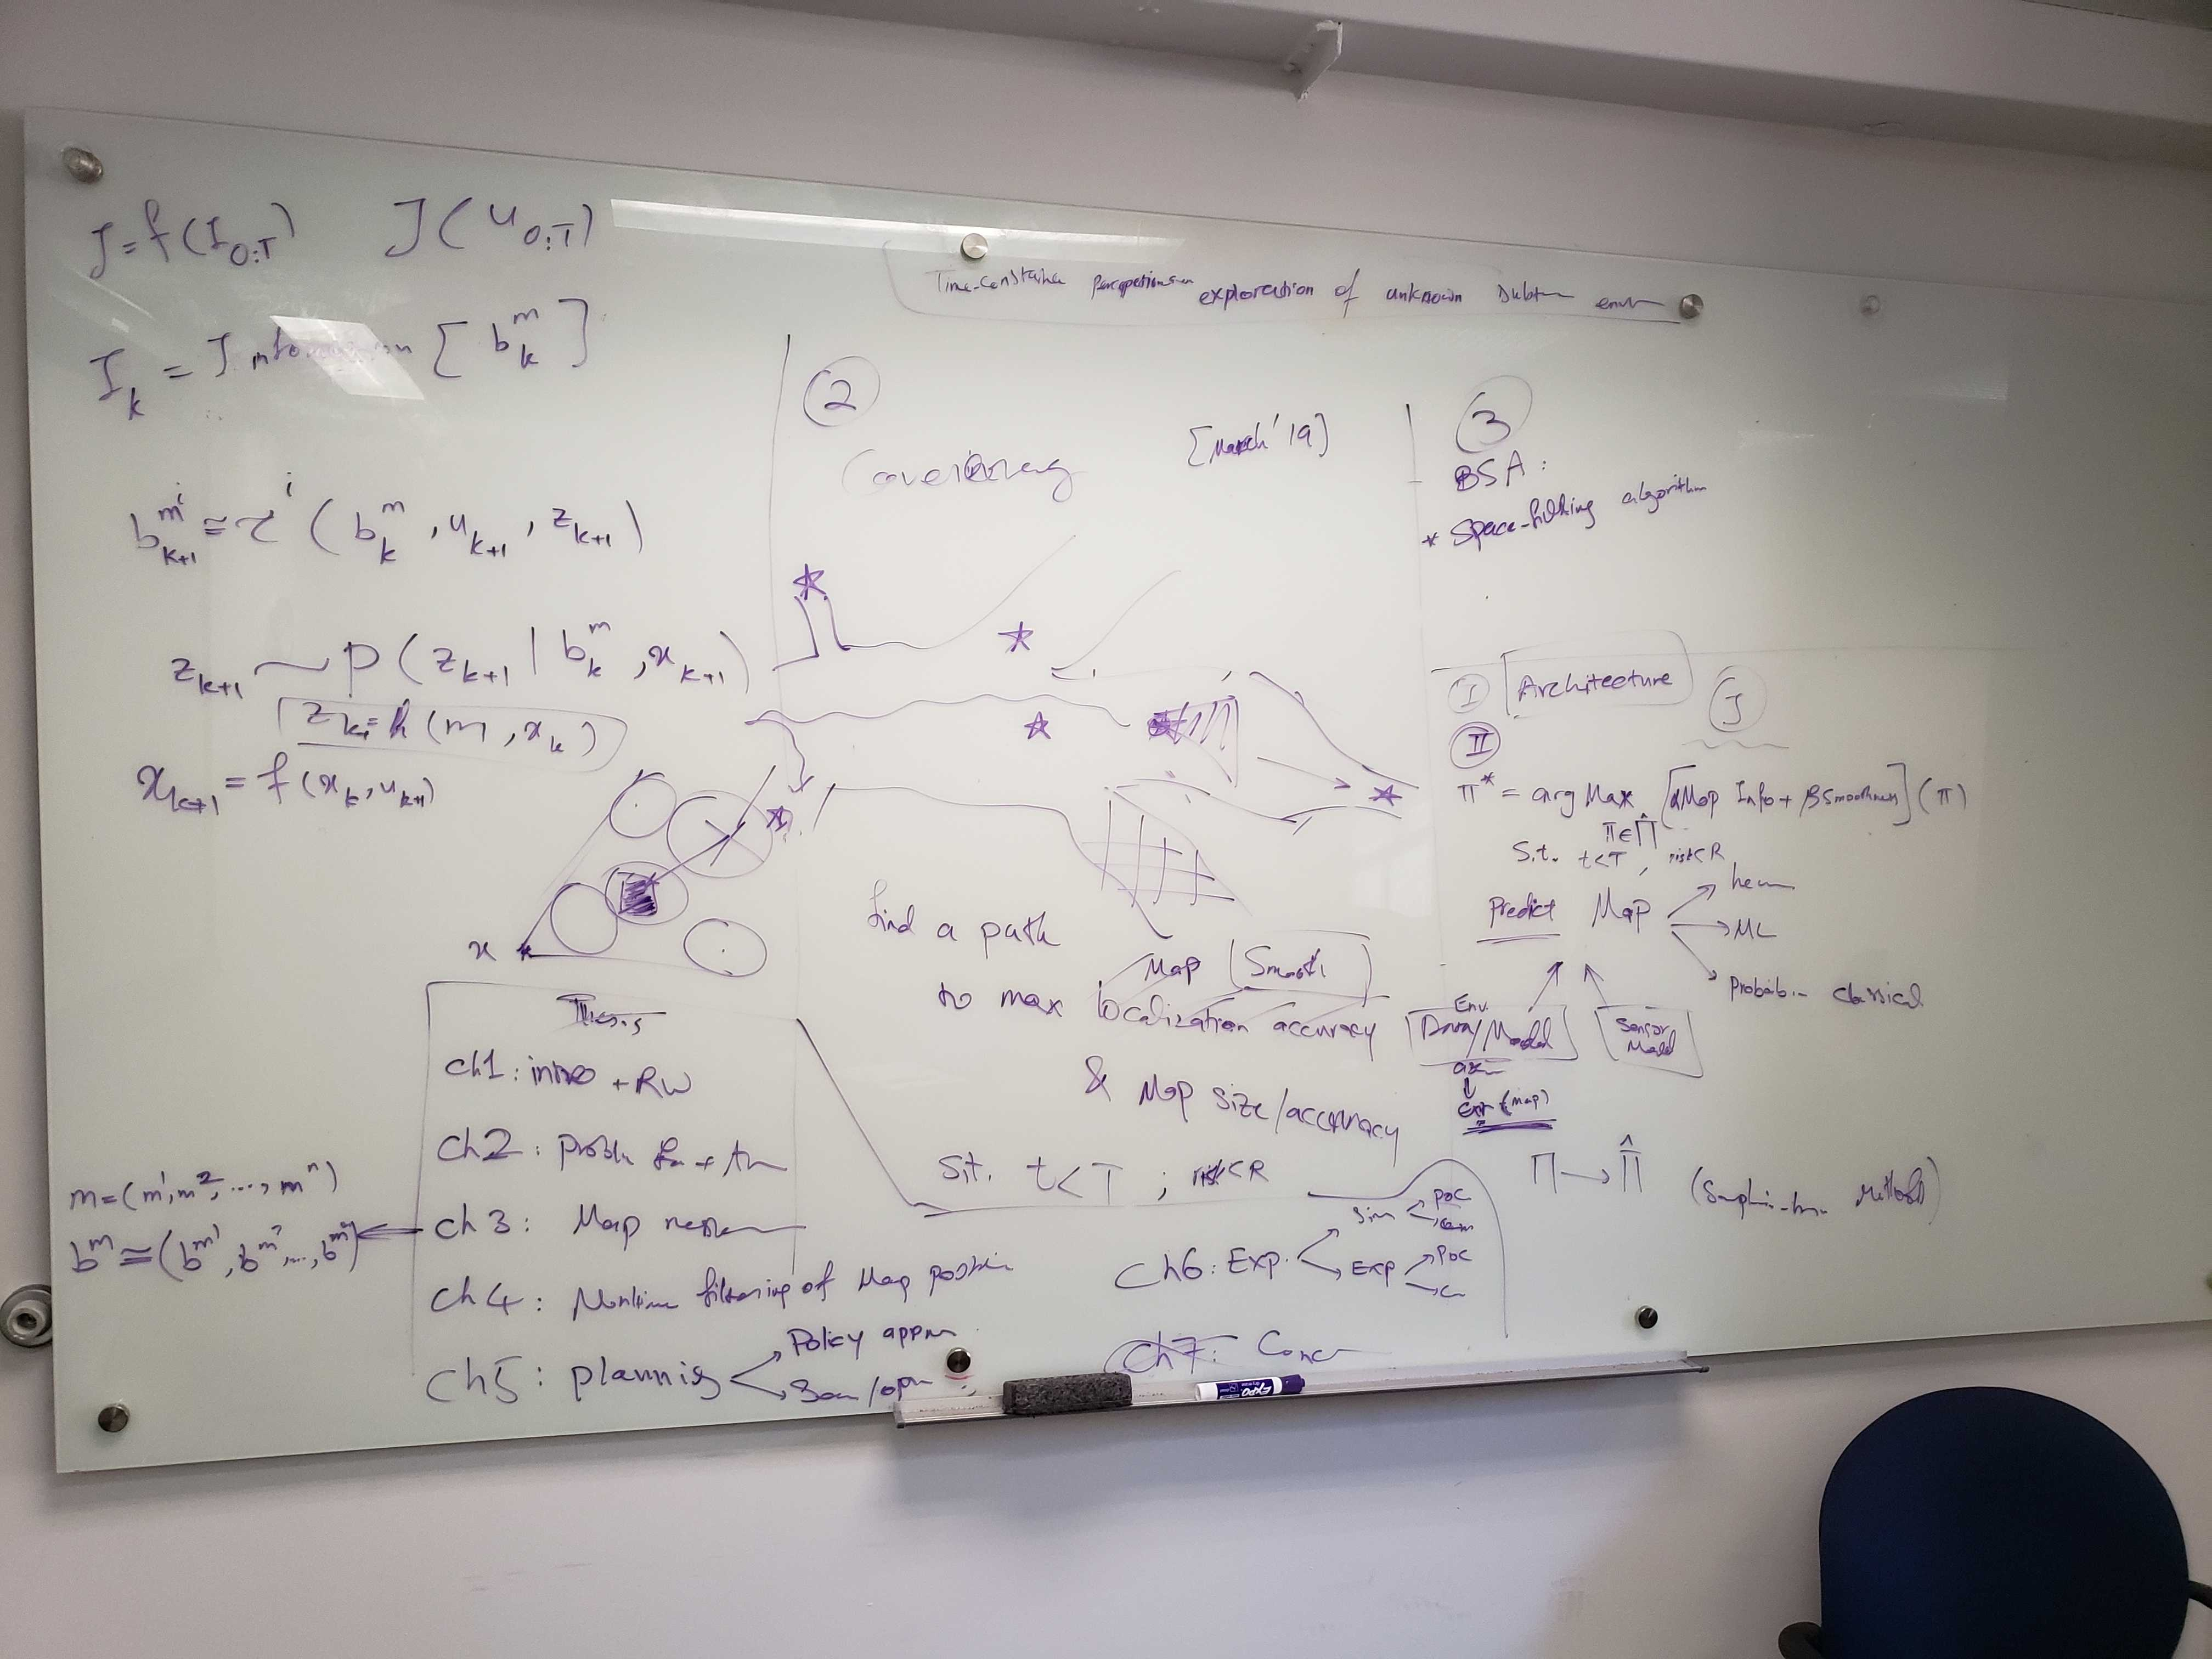
\includegraphics[width=.5\textwidth]{figures/whiteboard1.jpg}
  \label{fig:whiteboard1}
\end{figure}

\begin{figure}[H]
  \centering
  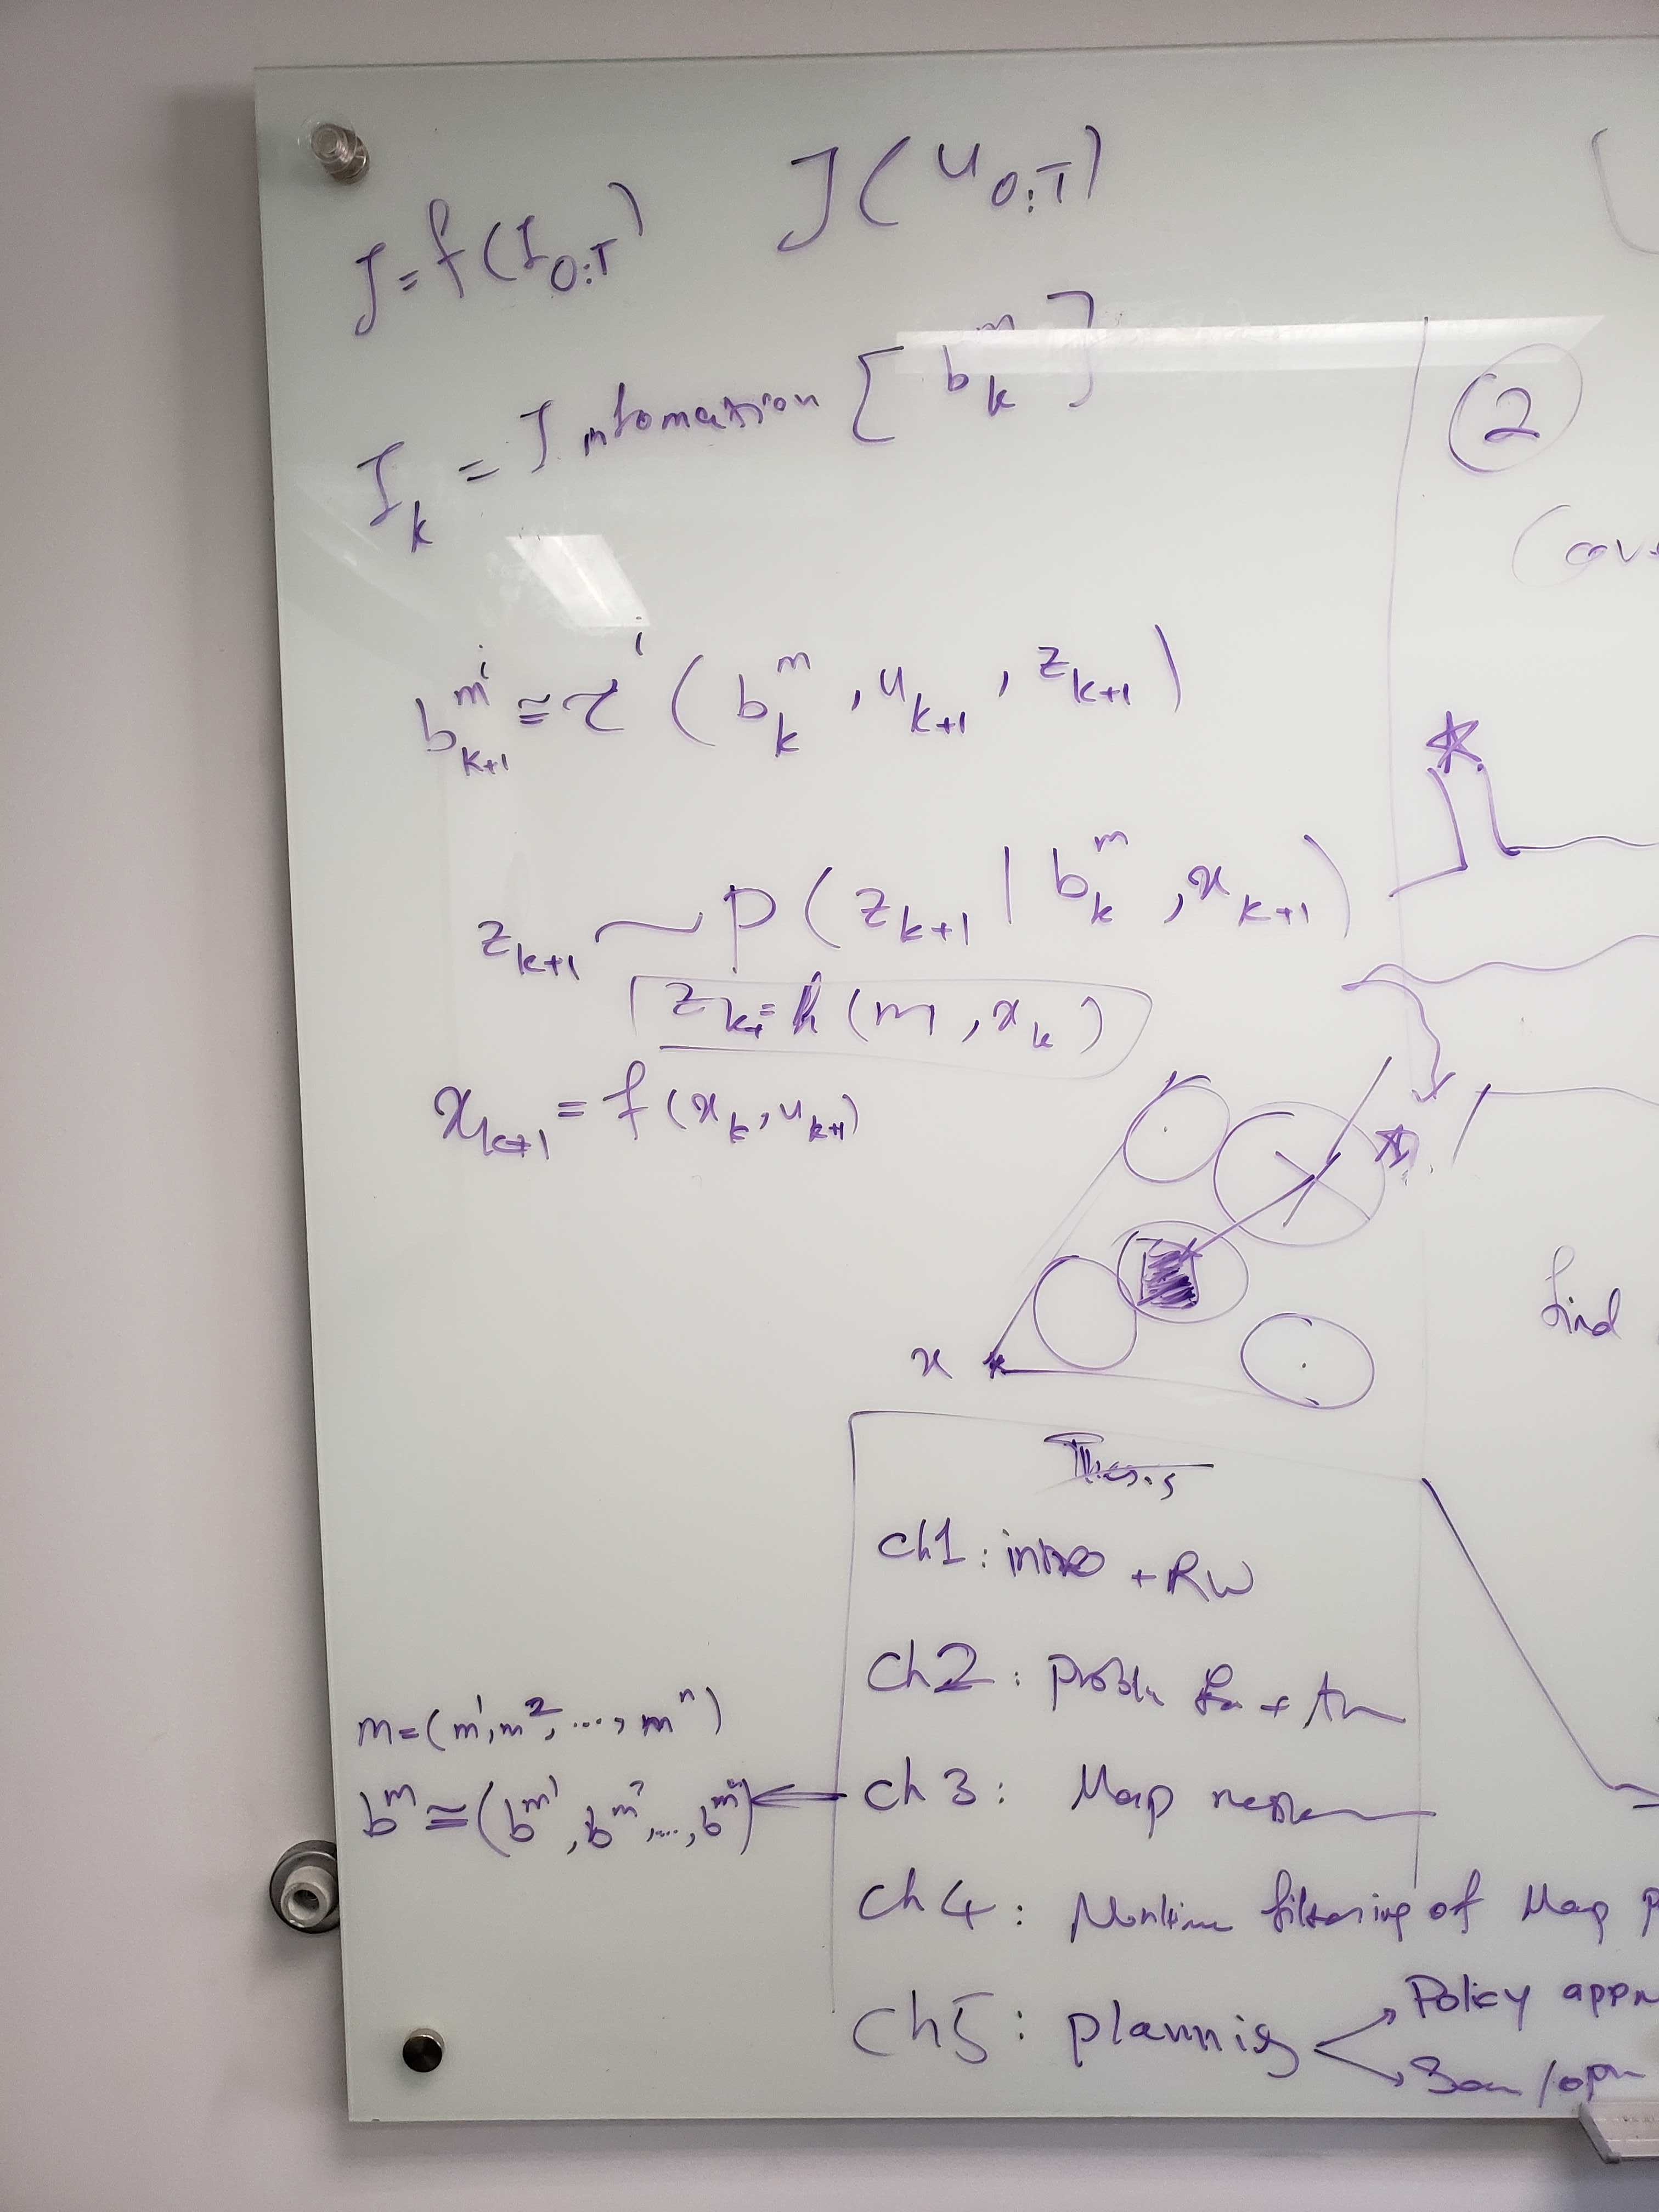
\includegraphics[width=.5\textwidth]{figures/whiteboard2.jpg}
  \label{fig:whiteboard1}
\end{figure}

\begin{figure}[H]
  \centering
  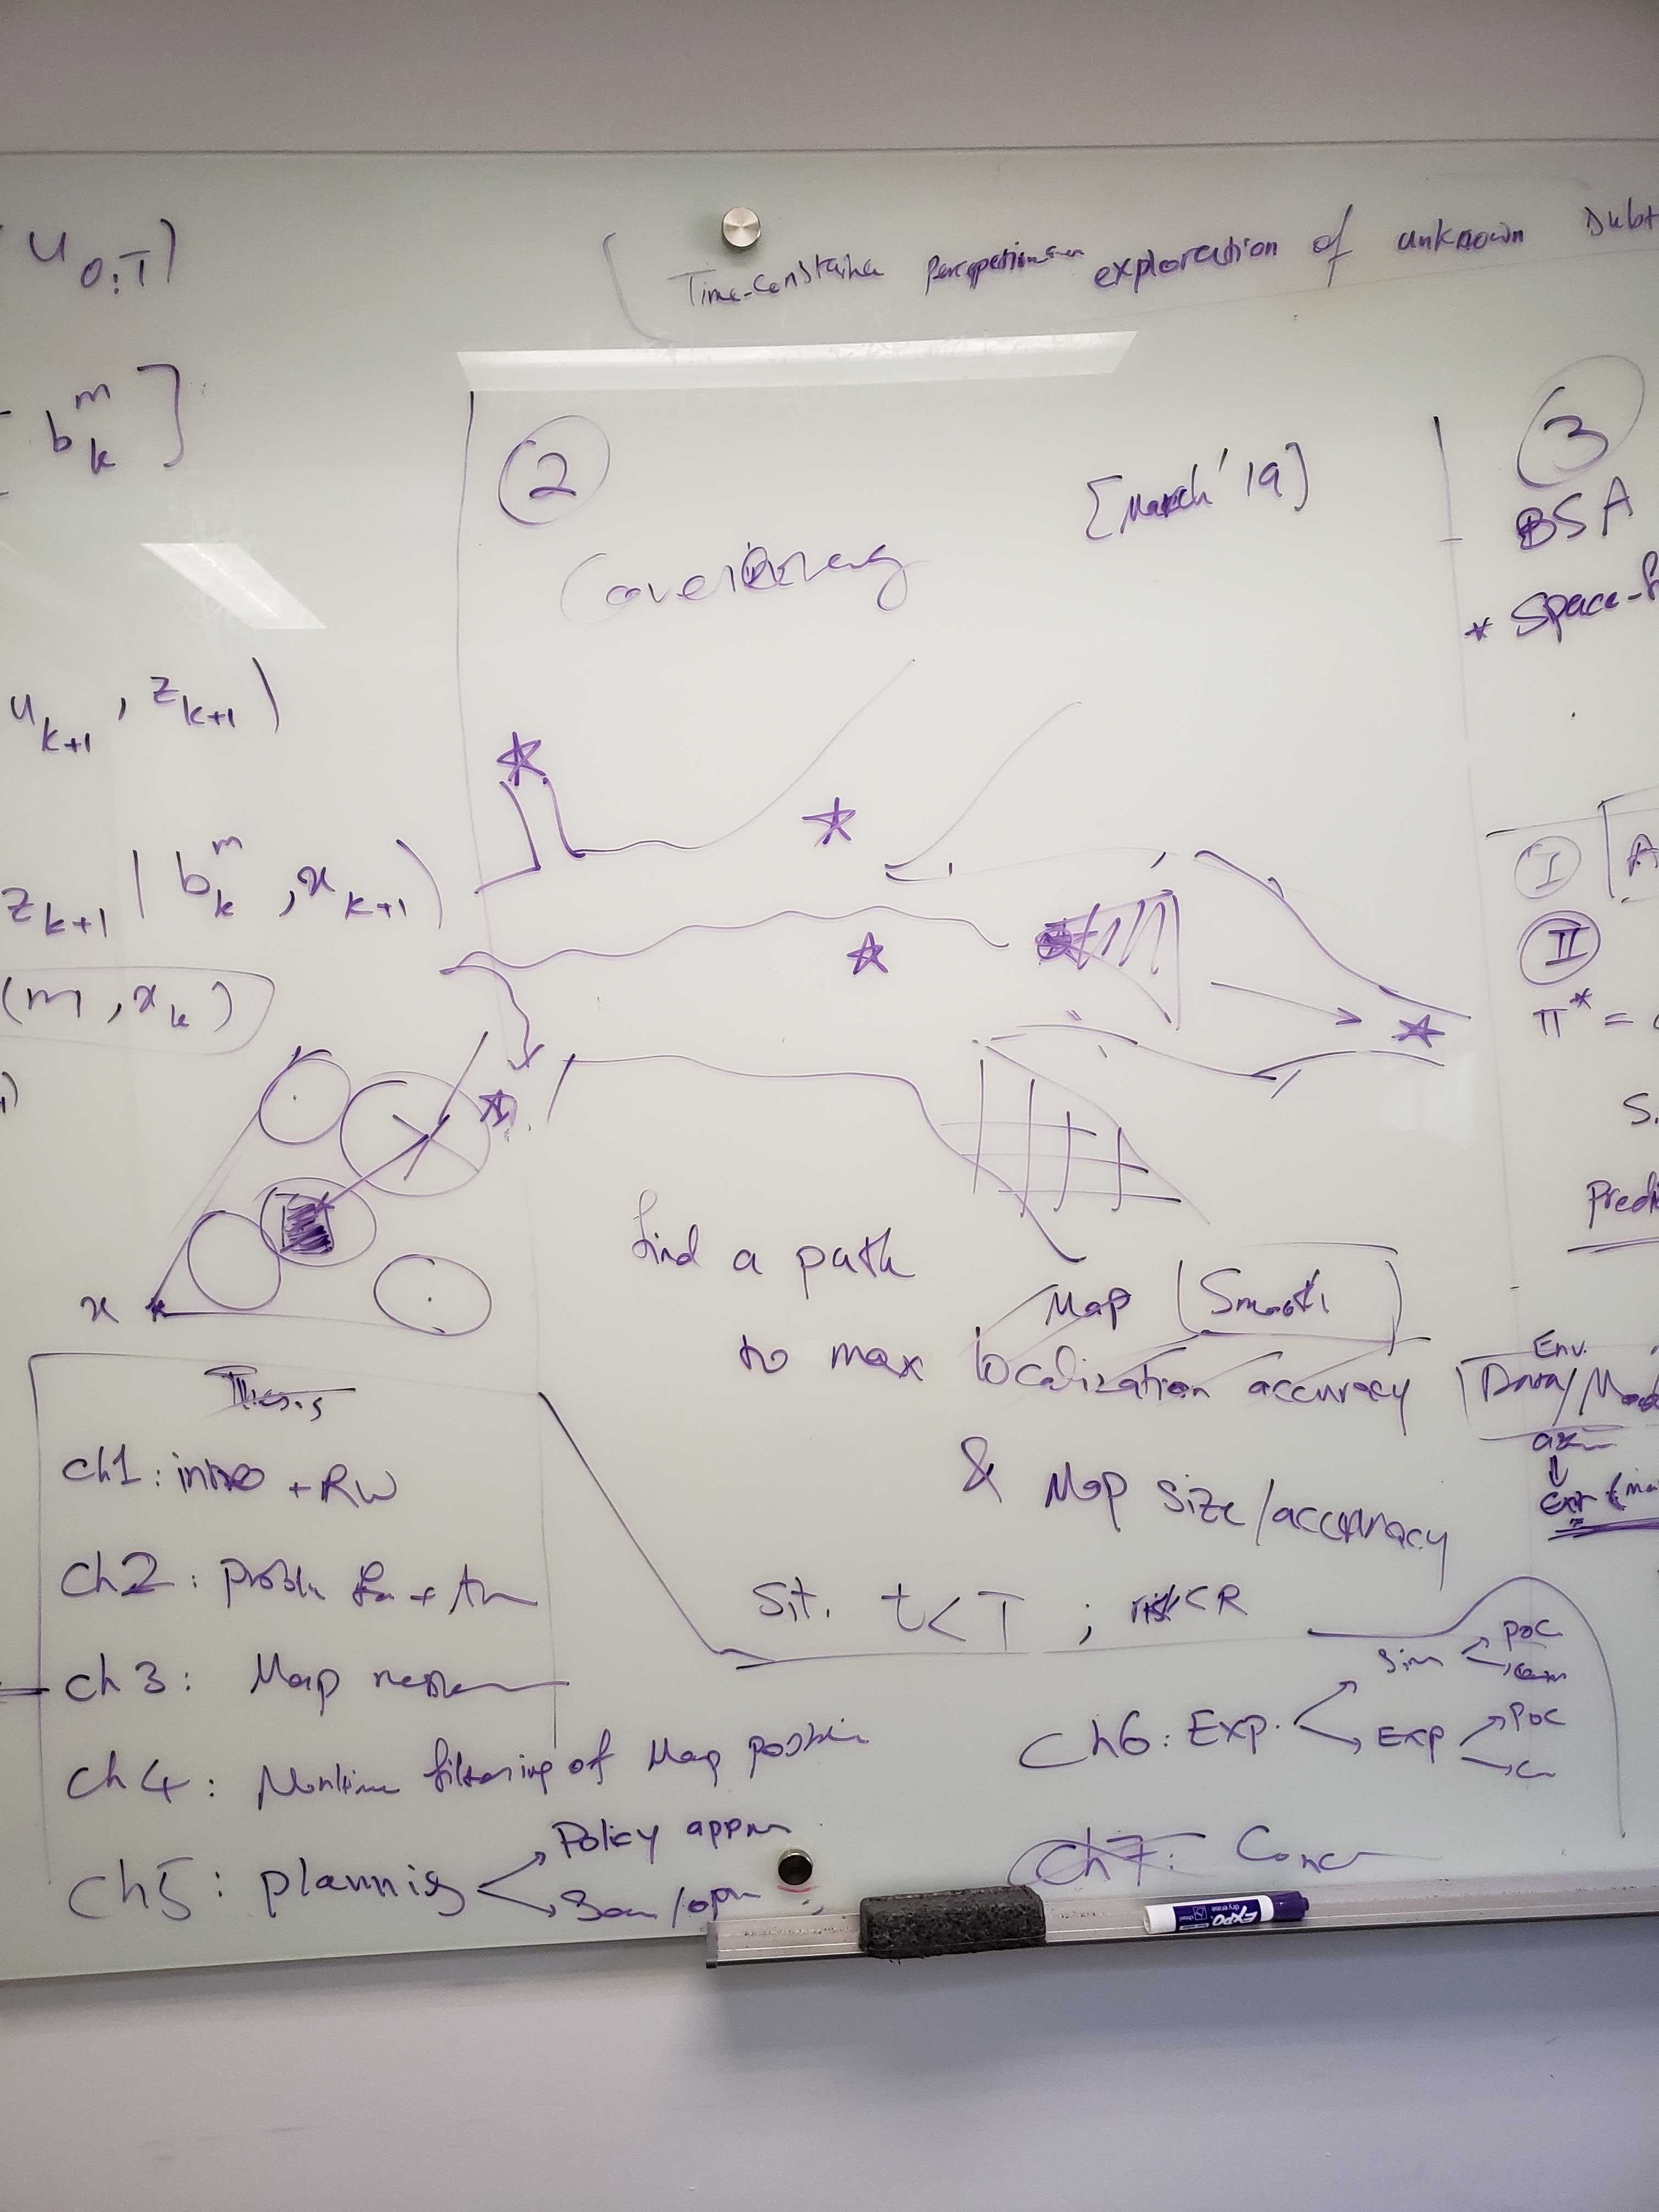
\includegraphics[width=.5\textwidth]{figures/whiteboard3.jpg}
  \label{fig:whiteboard1}
\end{figure}

\begin{figure}[H]
  \centering
  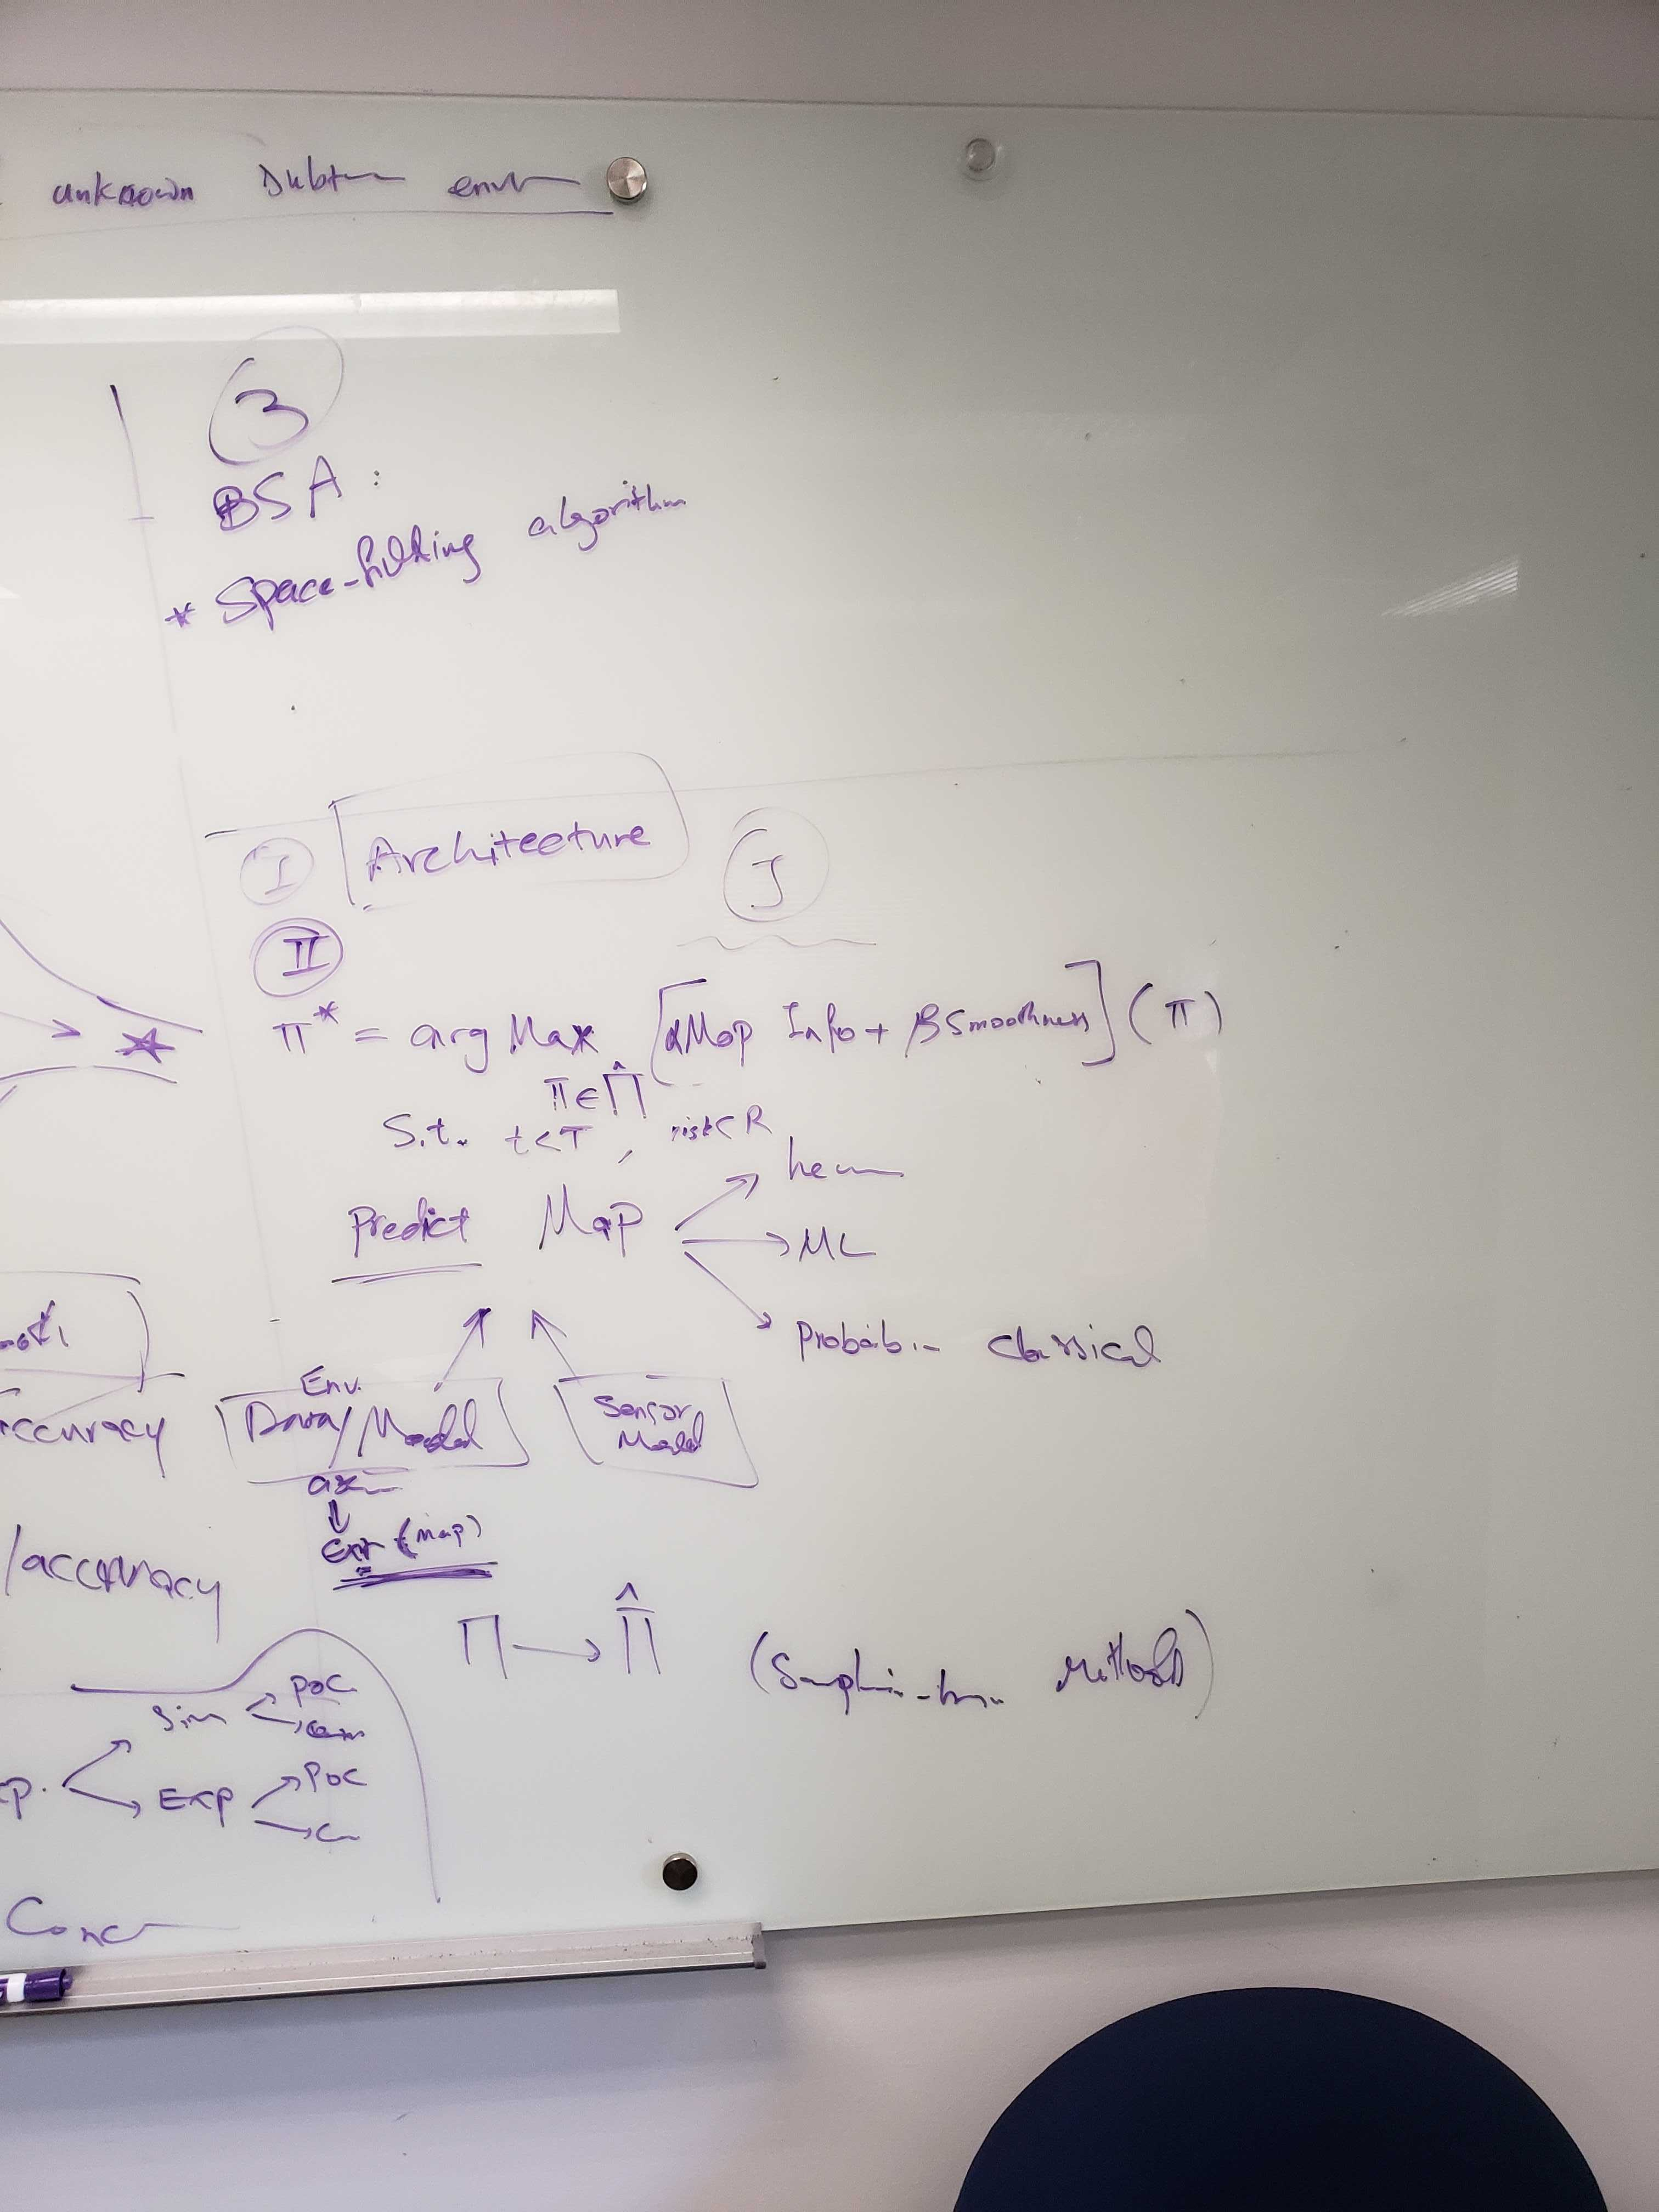
\includegraphics[width=.5\textwidth]{figures/whiteboard4.jpg}
  \label{fig:whiteboard1}
\end{figure}

\clearpage
\begin{figure}[H]
  \centering
  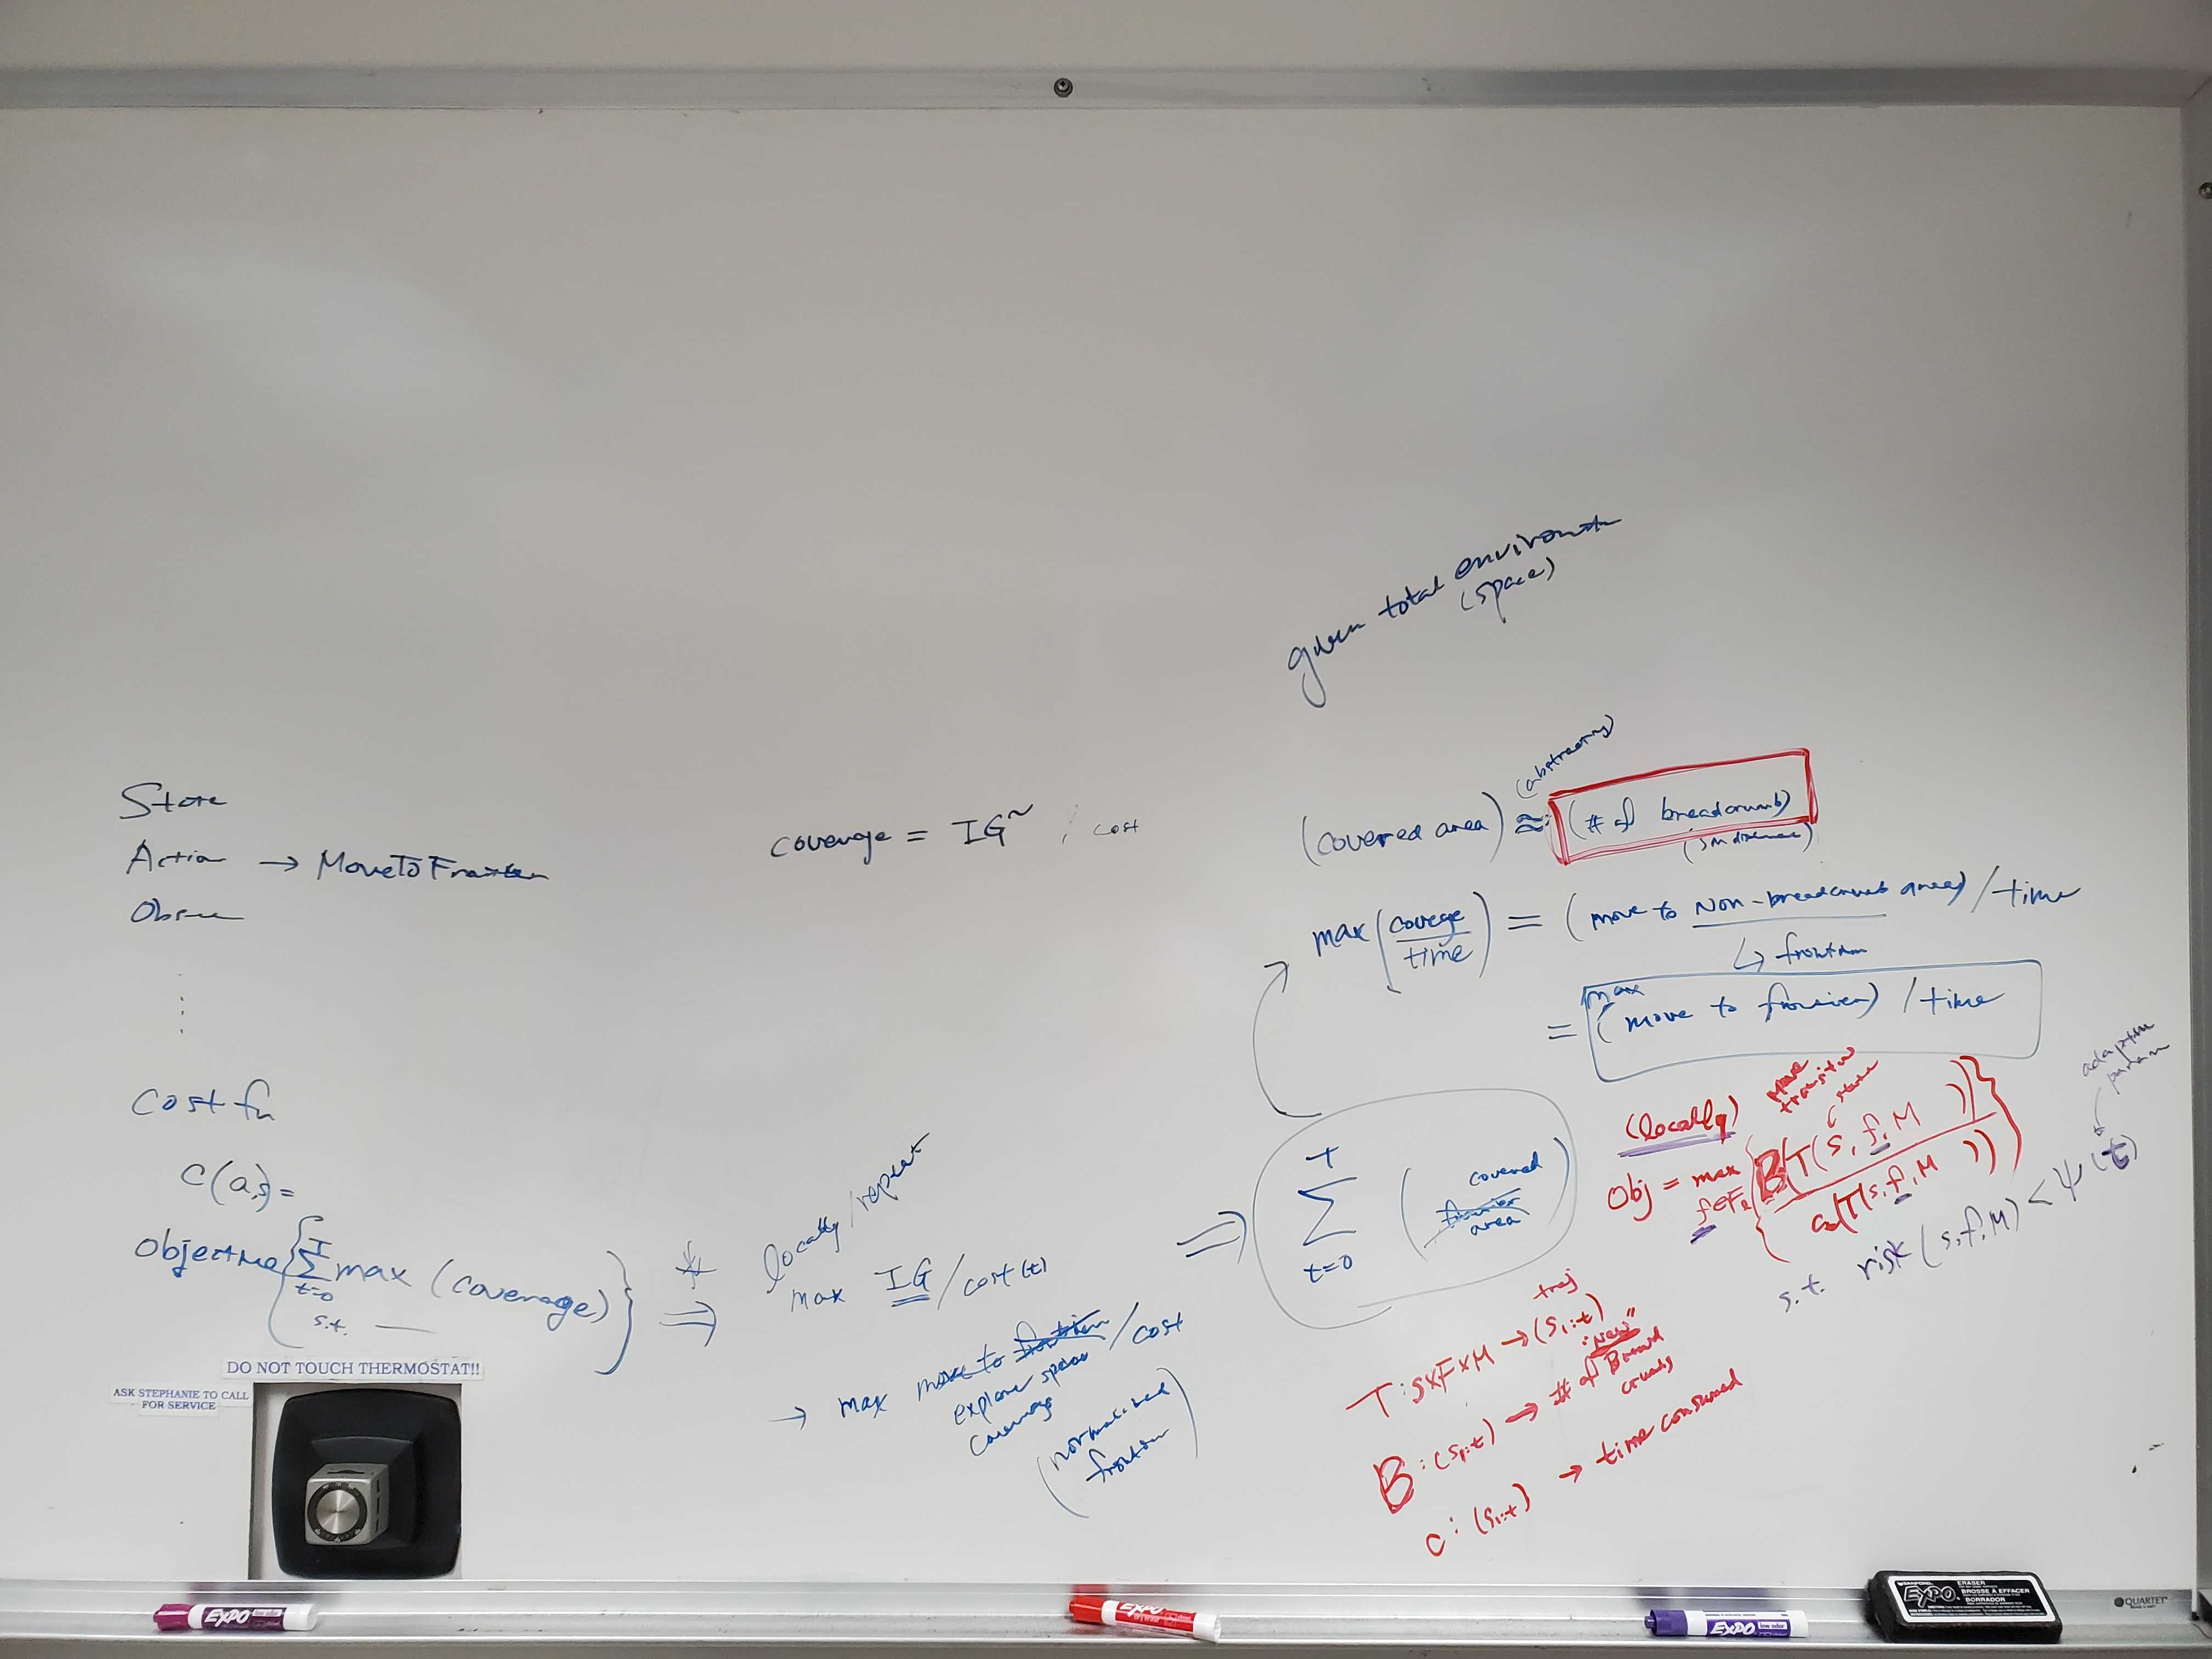
\includegraphics[width=.9\textwidth]{figures/whiteboardA.jpg}
  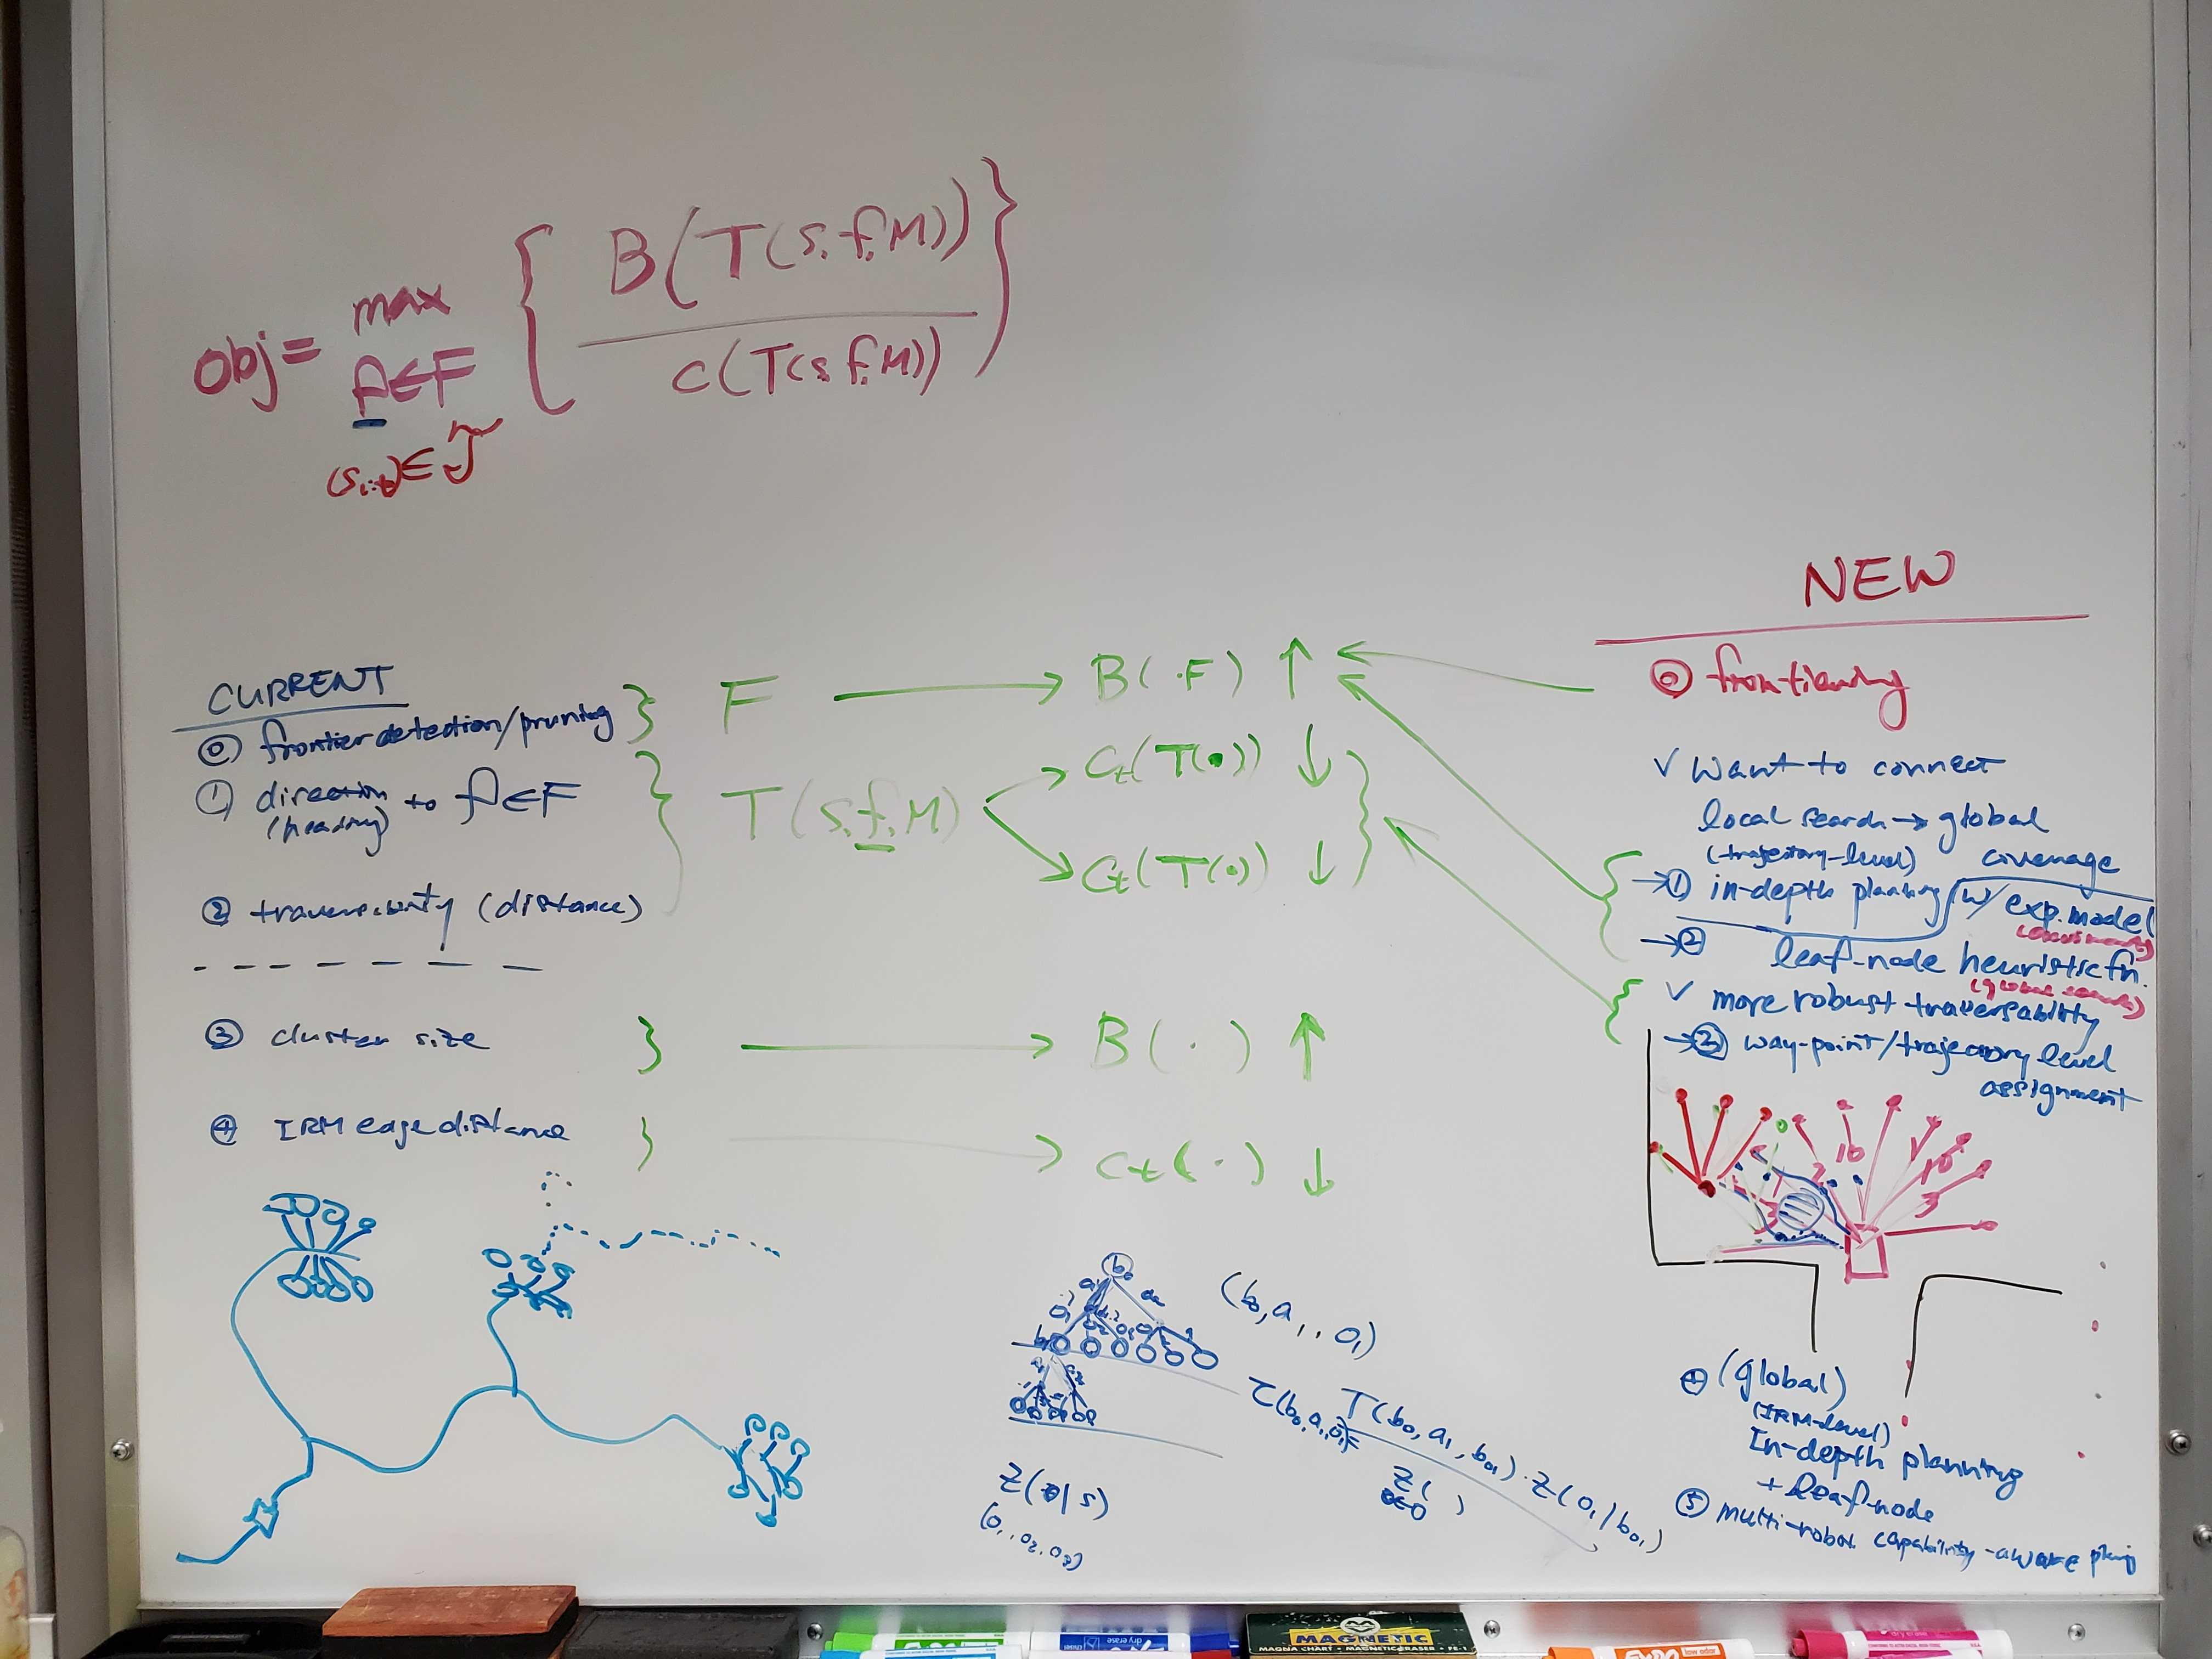
\includegraphics[width=.9\textwidth]{figures/whiteboardB.jpg}
\end{figure}
\clearpage

\clearpage
\begin{figure}[H]
  \centering
  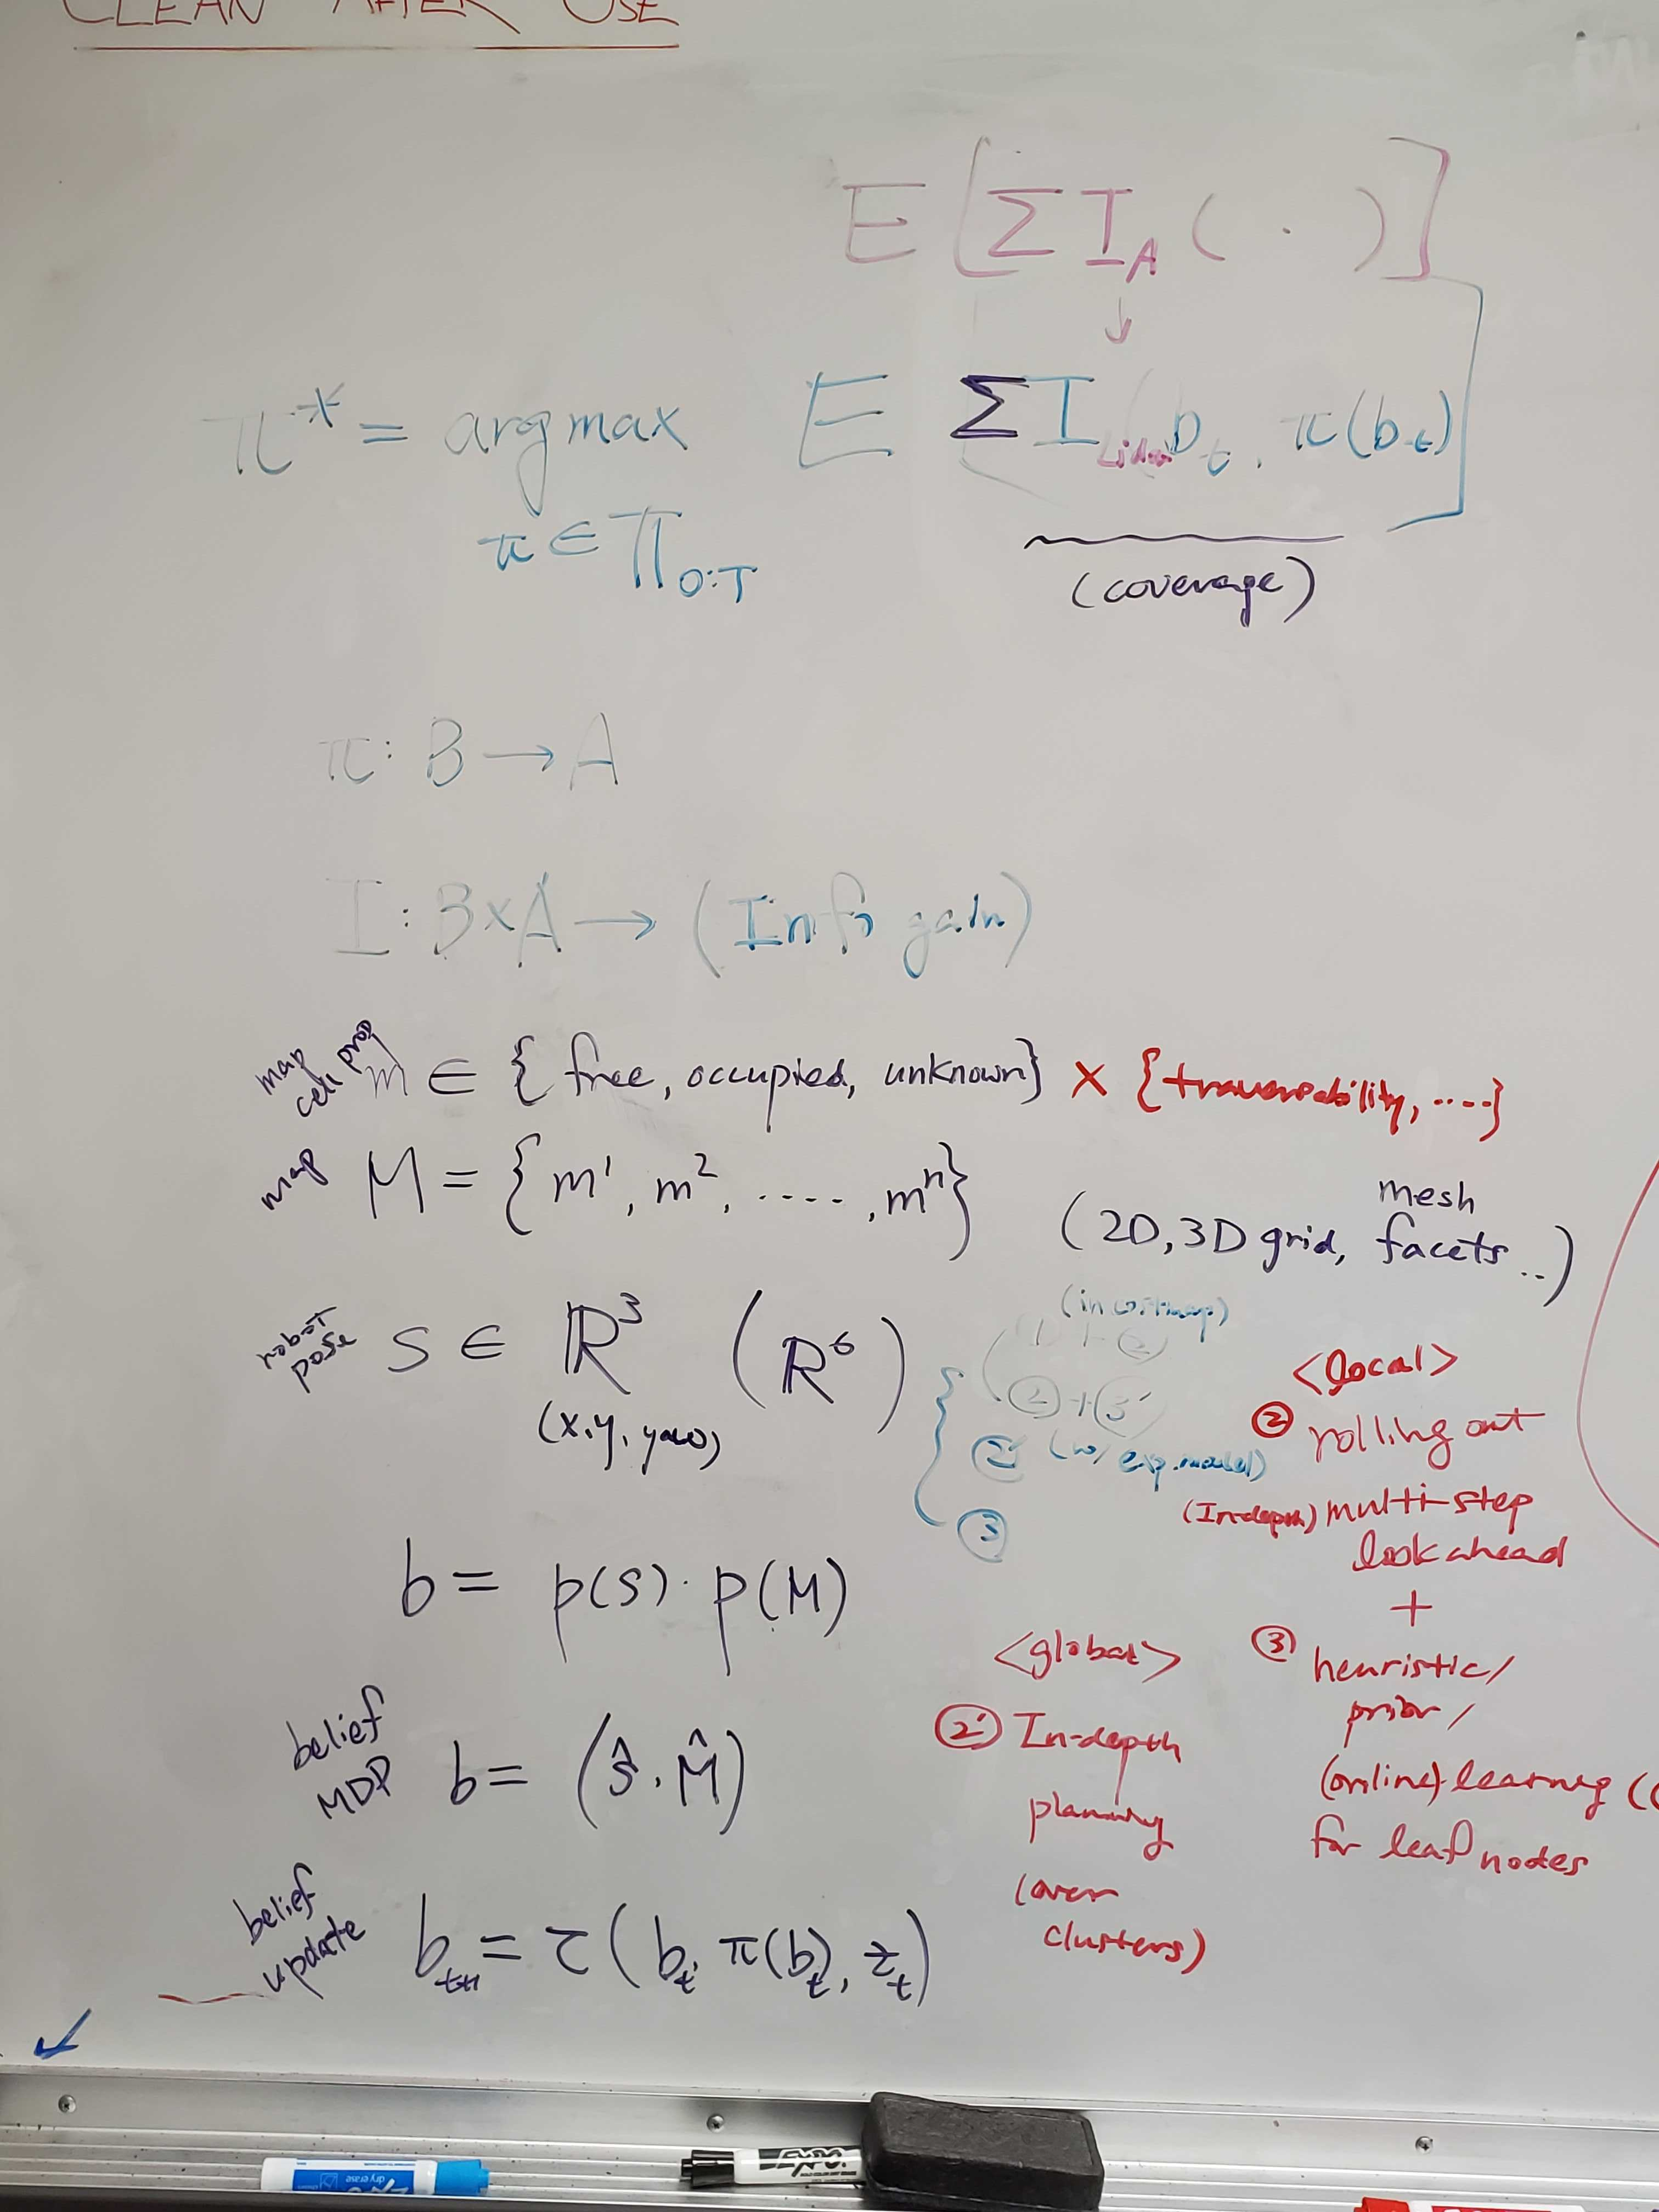
\includegraphics[width=.9\textwidth]{figures/whiteboardI.jpg}
\end{figure}
\clearpage
\begin{figure}[H]
  \centering
  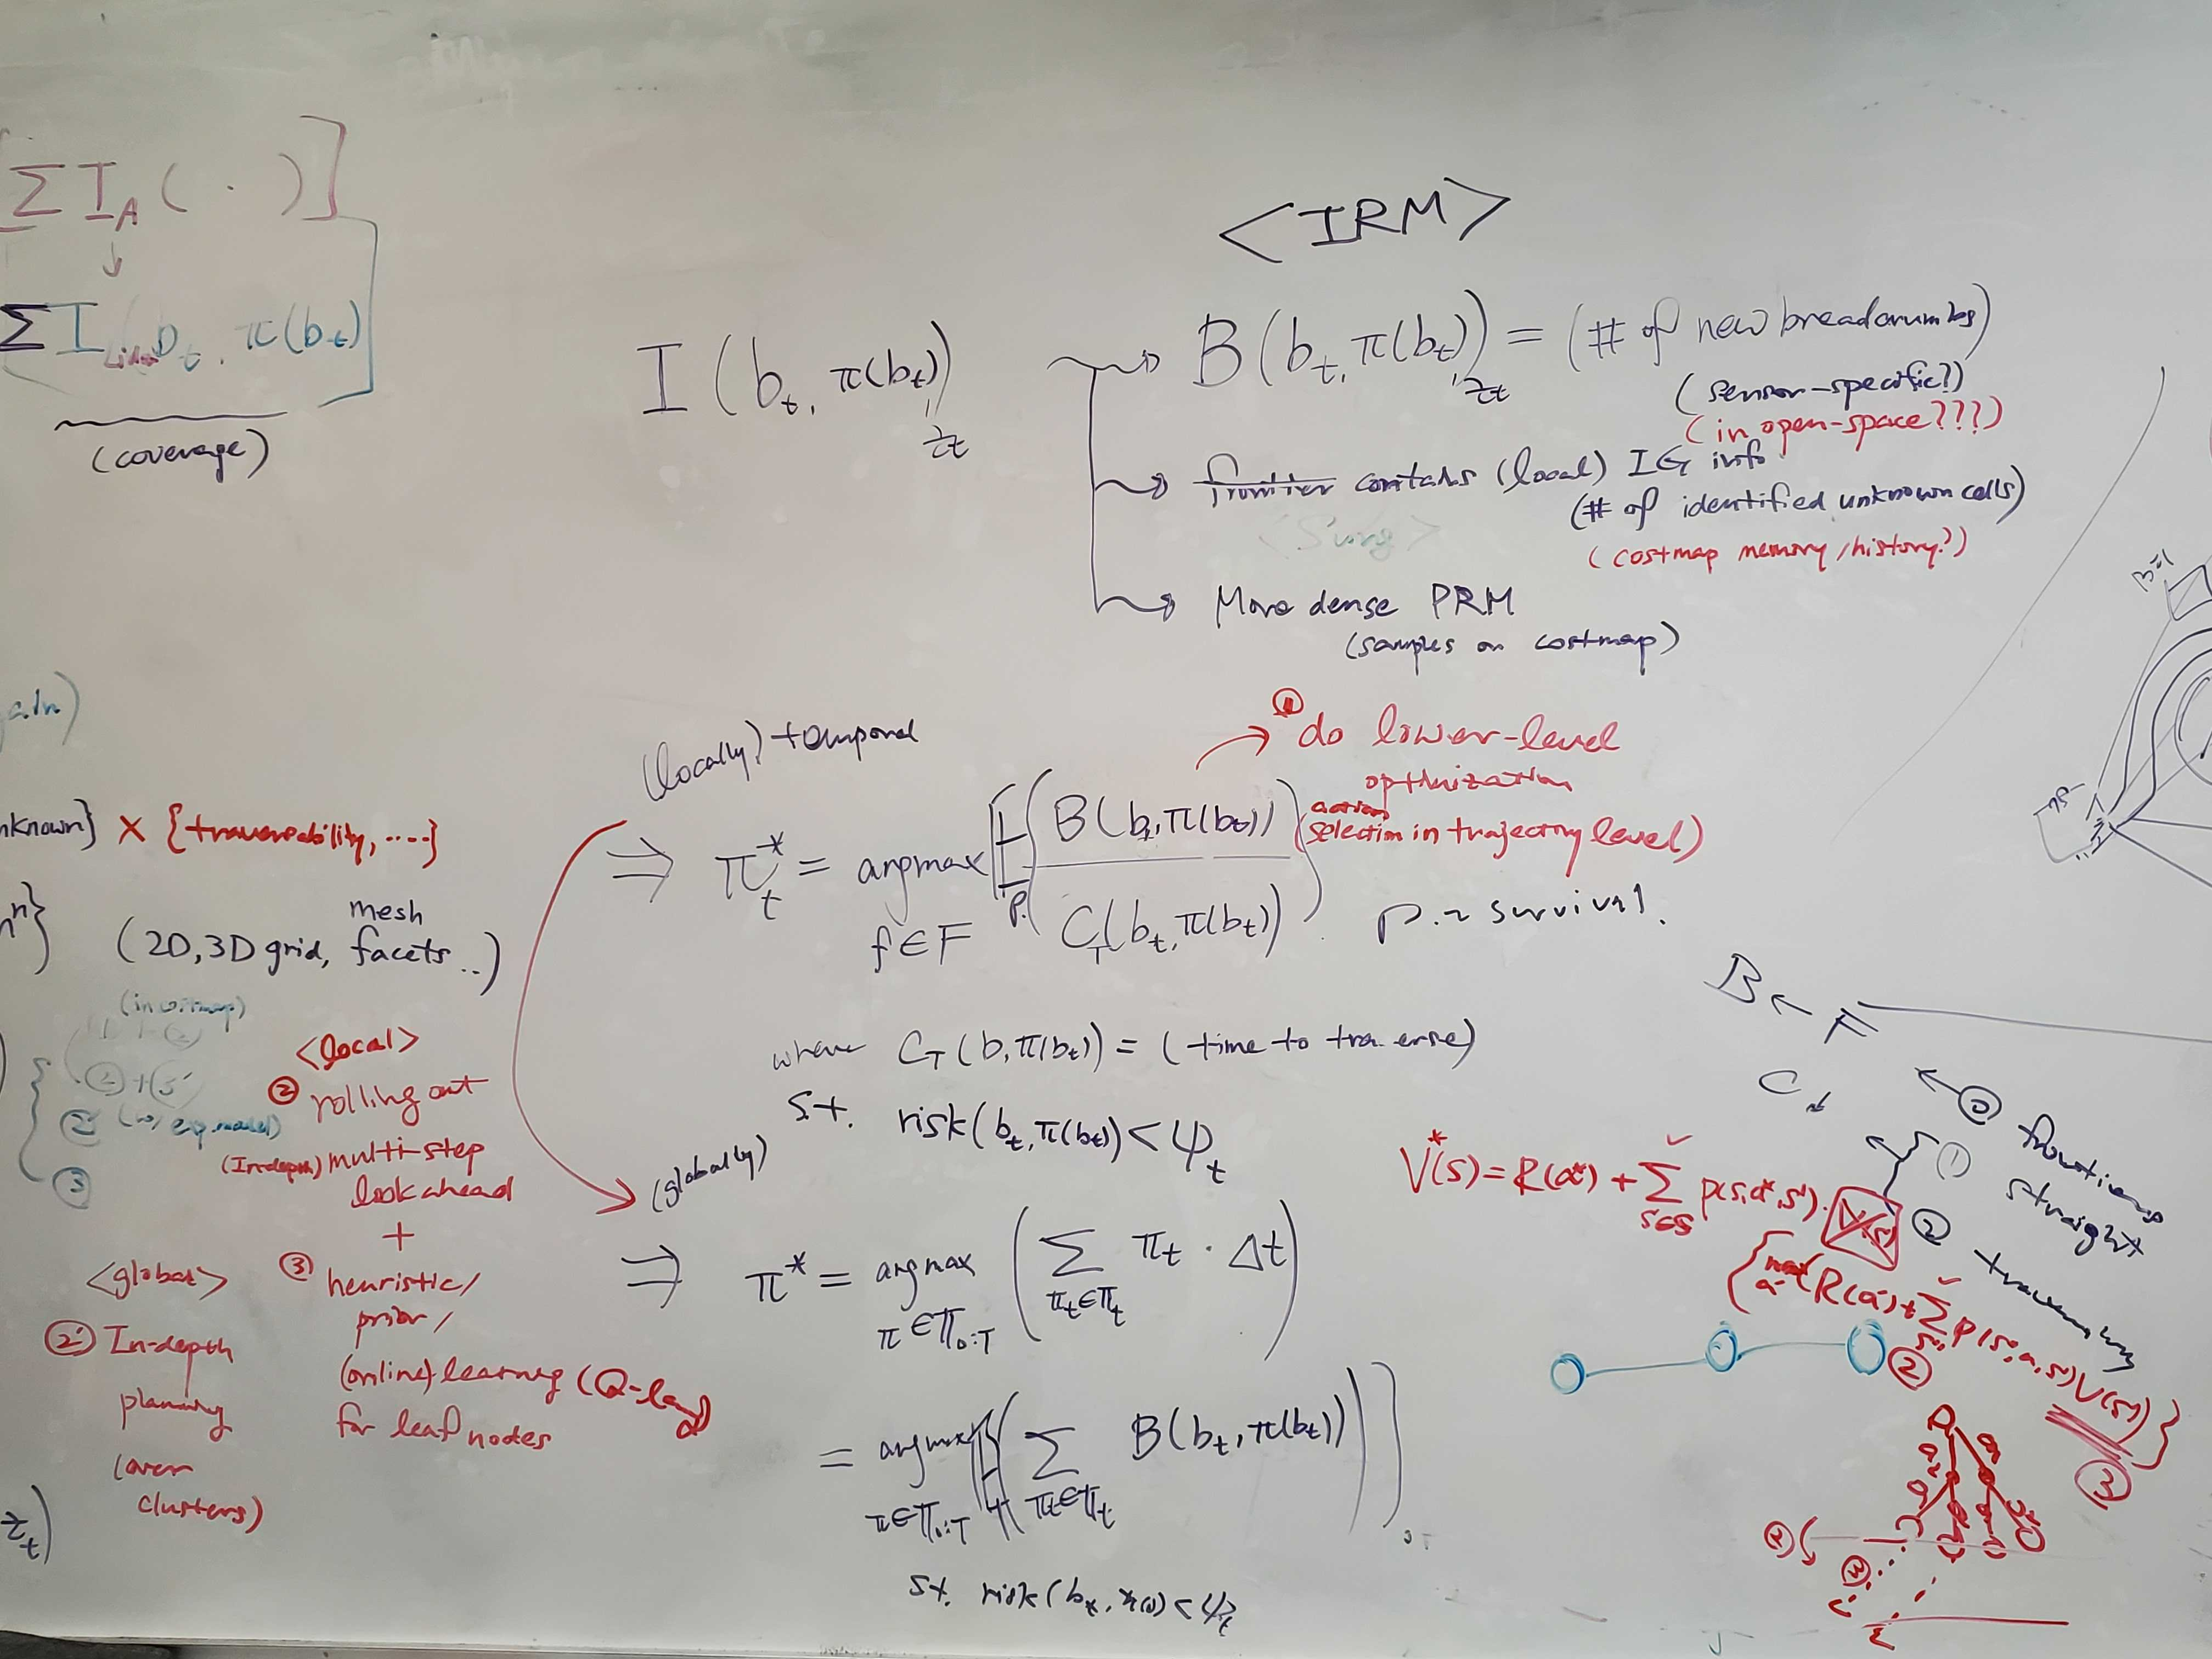
\includegraphics[width=.9\textwidth]{figures/whiteboardII.jpg}
  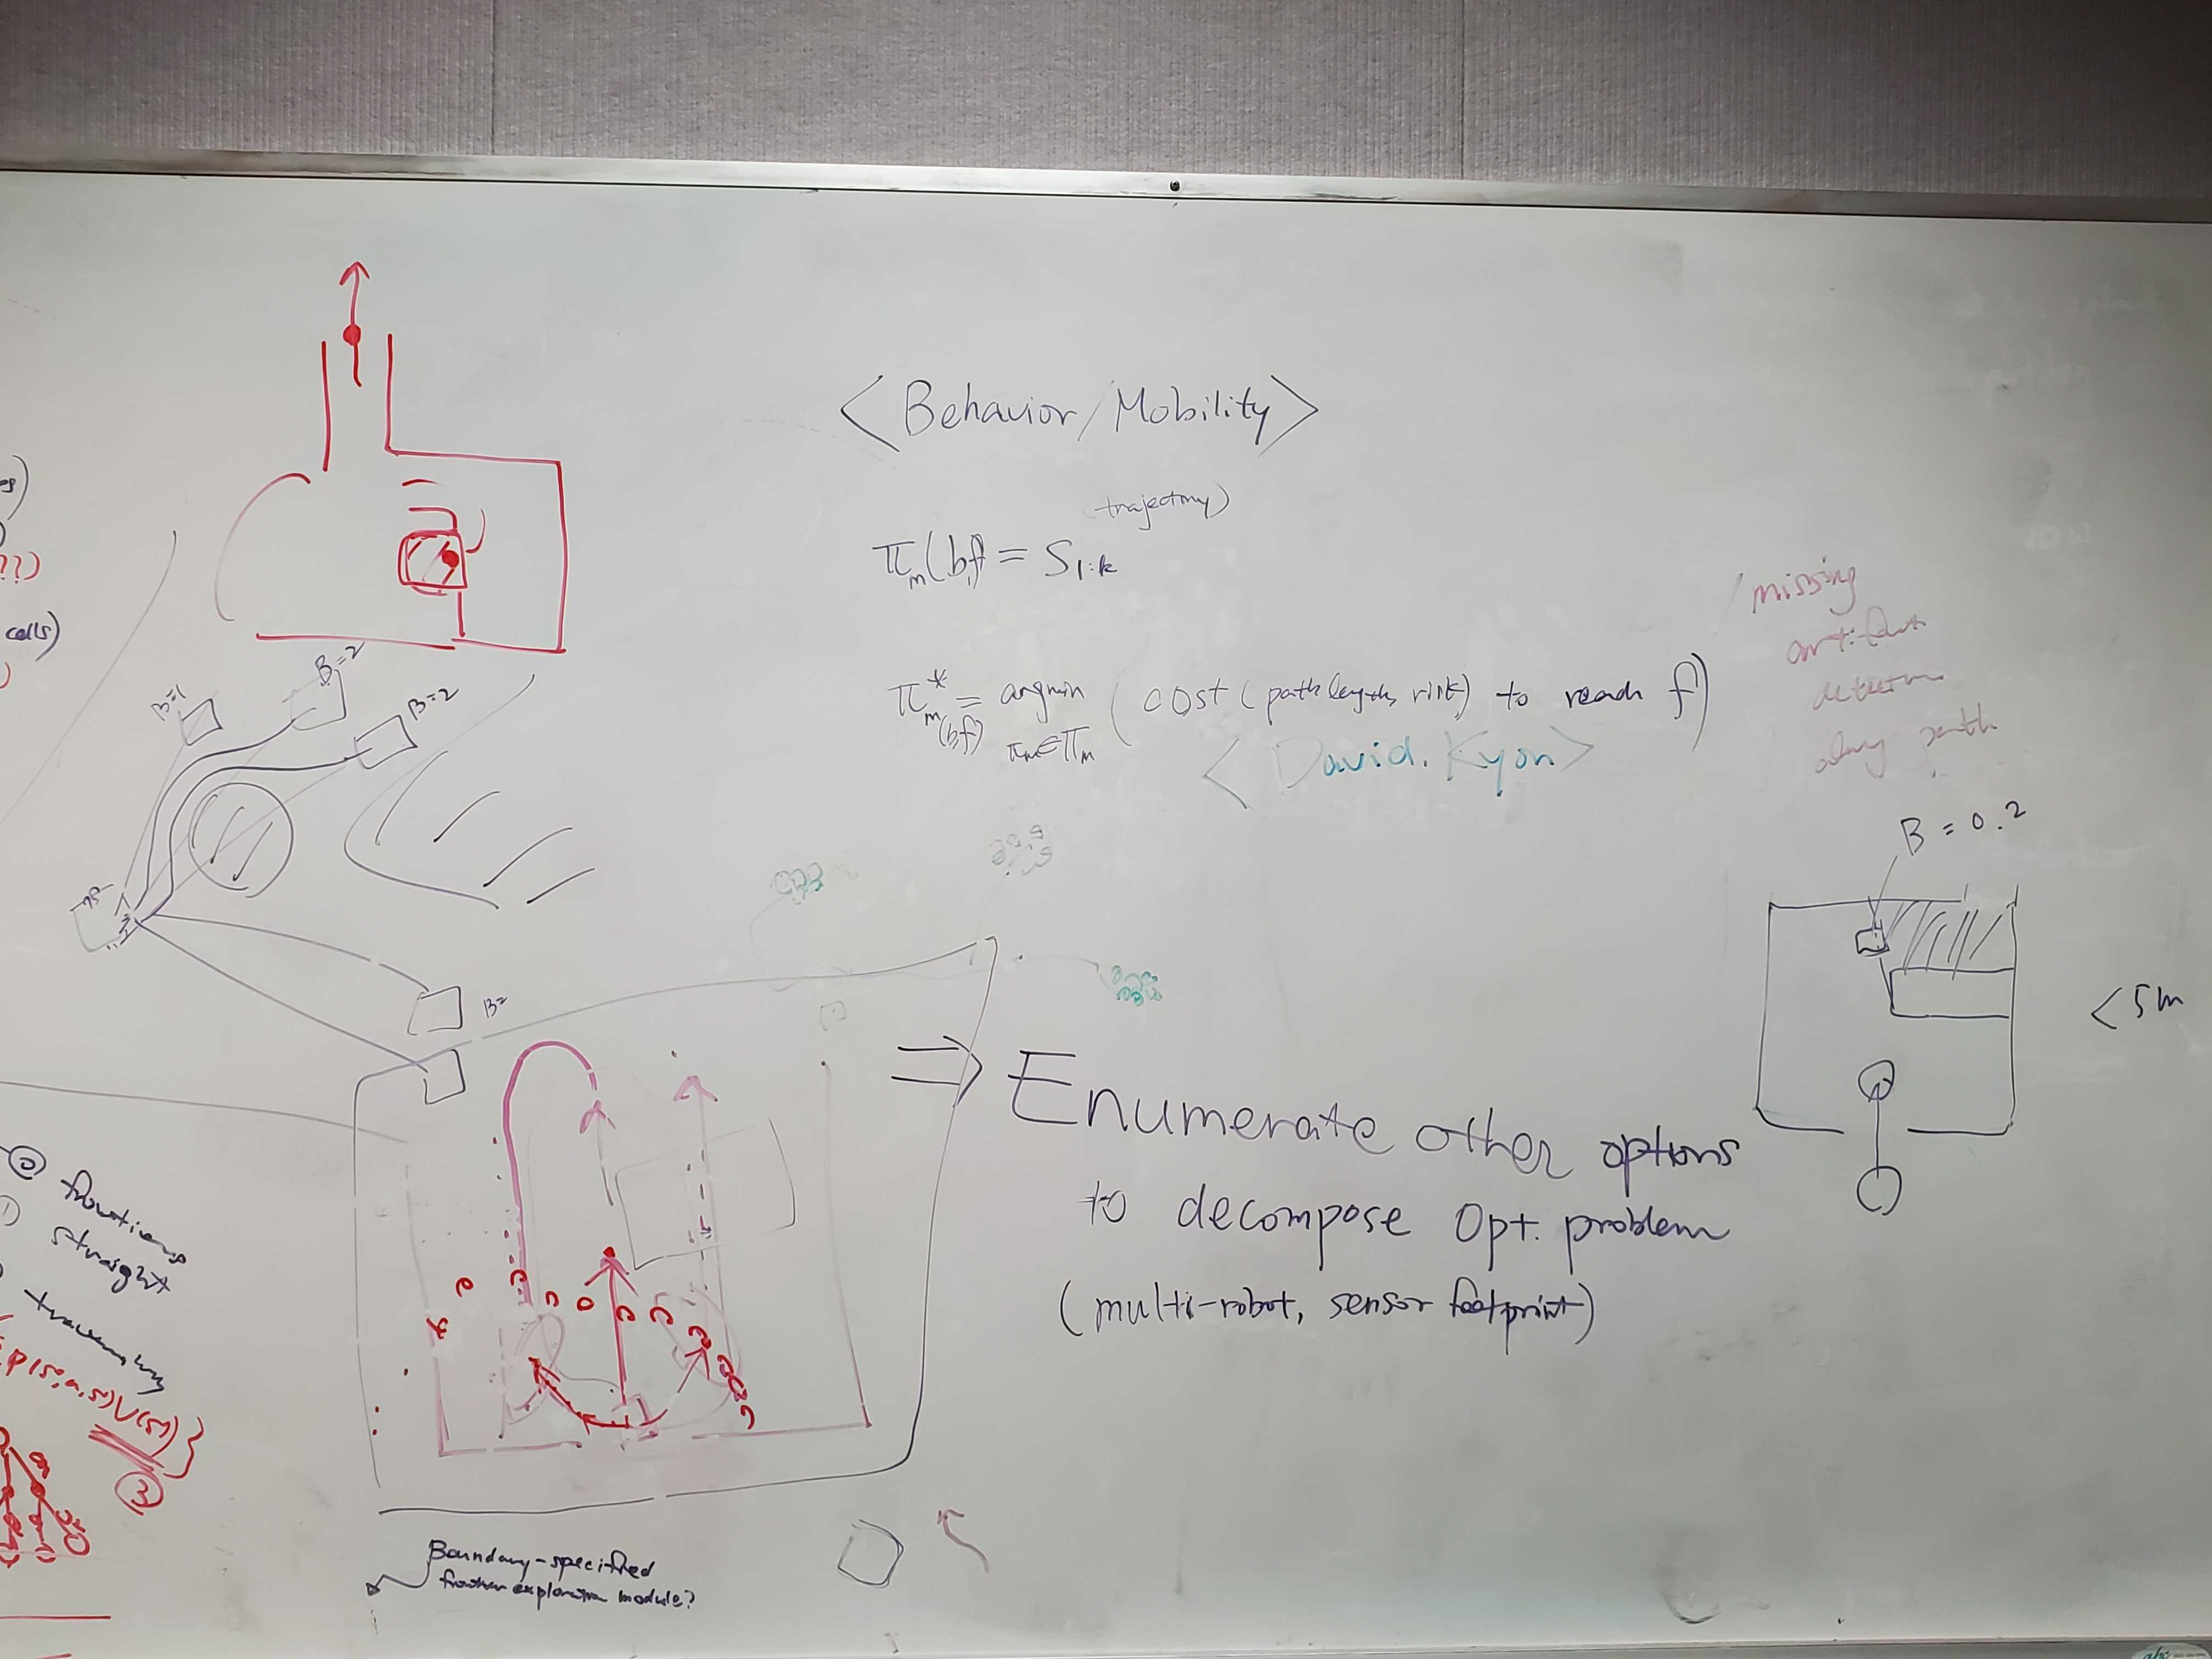
\includegraphics[width=.9\textwidth]{figures/whiteboardIII.jpg}
\end{figure}
\clearpage


\end{document}
